\documentclass[12pt,a4paper]{article}

%-------------------Packages-------------------%
\input Acorn.fd
\usepackage[magyar]{babel}
\usepackage[T1]{fontenc}
\usepackage{kpfonts}
\usepackage{changepage}
\usepackage{xcolor}
\usepackage{tikz}
\usepackage{wrapfig}
\usepackage{hyperref}
\usepackage{fancyhdr}
\pagestyle{fancy}
\usepackage{anyfontsize,lettrine}
\usepackage{pdfpages}
\usepackage{listings}
\usepackage{tcolorbox}

%-------------------Settings-------------------%
\graphicspath{{./images/}}
\setlength\parindent{0pt}


\cfoot{}

\lhead{\rightmark}
\rhead{\thepage}
\setcounter{DefaultLines}{3}

%-------------------Commands-------------------%
\newcommand{\AUTHOR}{Herőczi Sándor}
\newcommand{\NEPTUN}{WH0AMC}
\newcommand{\TITLE}{Mikrovezérlő alapú autonóm fegyverrendszer tervezése és fejlesztése}
\newcommand{\YEAR}{2024}
\newcommand{\LOCATION}{Budapest}
\newcommand{\ABRAKELL}{\textcolor{red}{IDE KELL MÉG ÁBRA}}
%-------------------Colours-------------------%
\definecolor{BMEbordo}{HTML}{862633}
\definecolor{light-gray}{gray}{0.95}

\newcommand{\code}[1]{\tcbox{\texttt{#1}}}
\newcommand{\w}[1]{\; \mathrm{#1}}
\newcommand{\q}[1]{\; \left[\mathrm{#1}\right]}

\tcbset{on line, 
	boxsep=4pt, left=0pt,right=0pt,top=0pt,bottom=0pt,
	colframe=white,colback=light-gray
}

\begin{document}

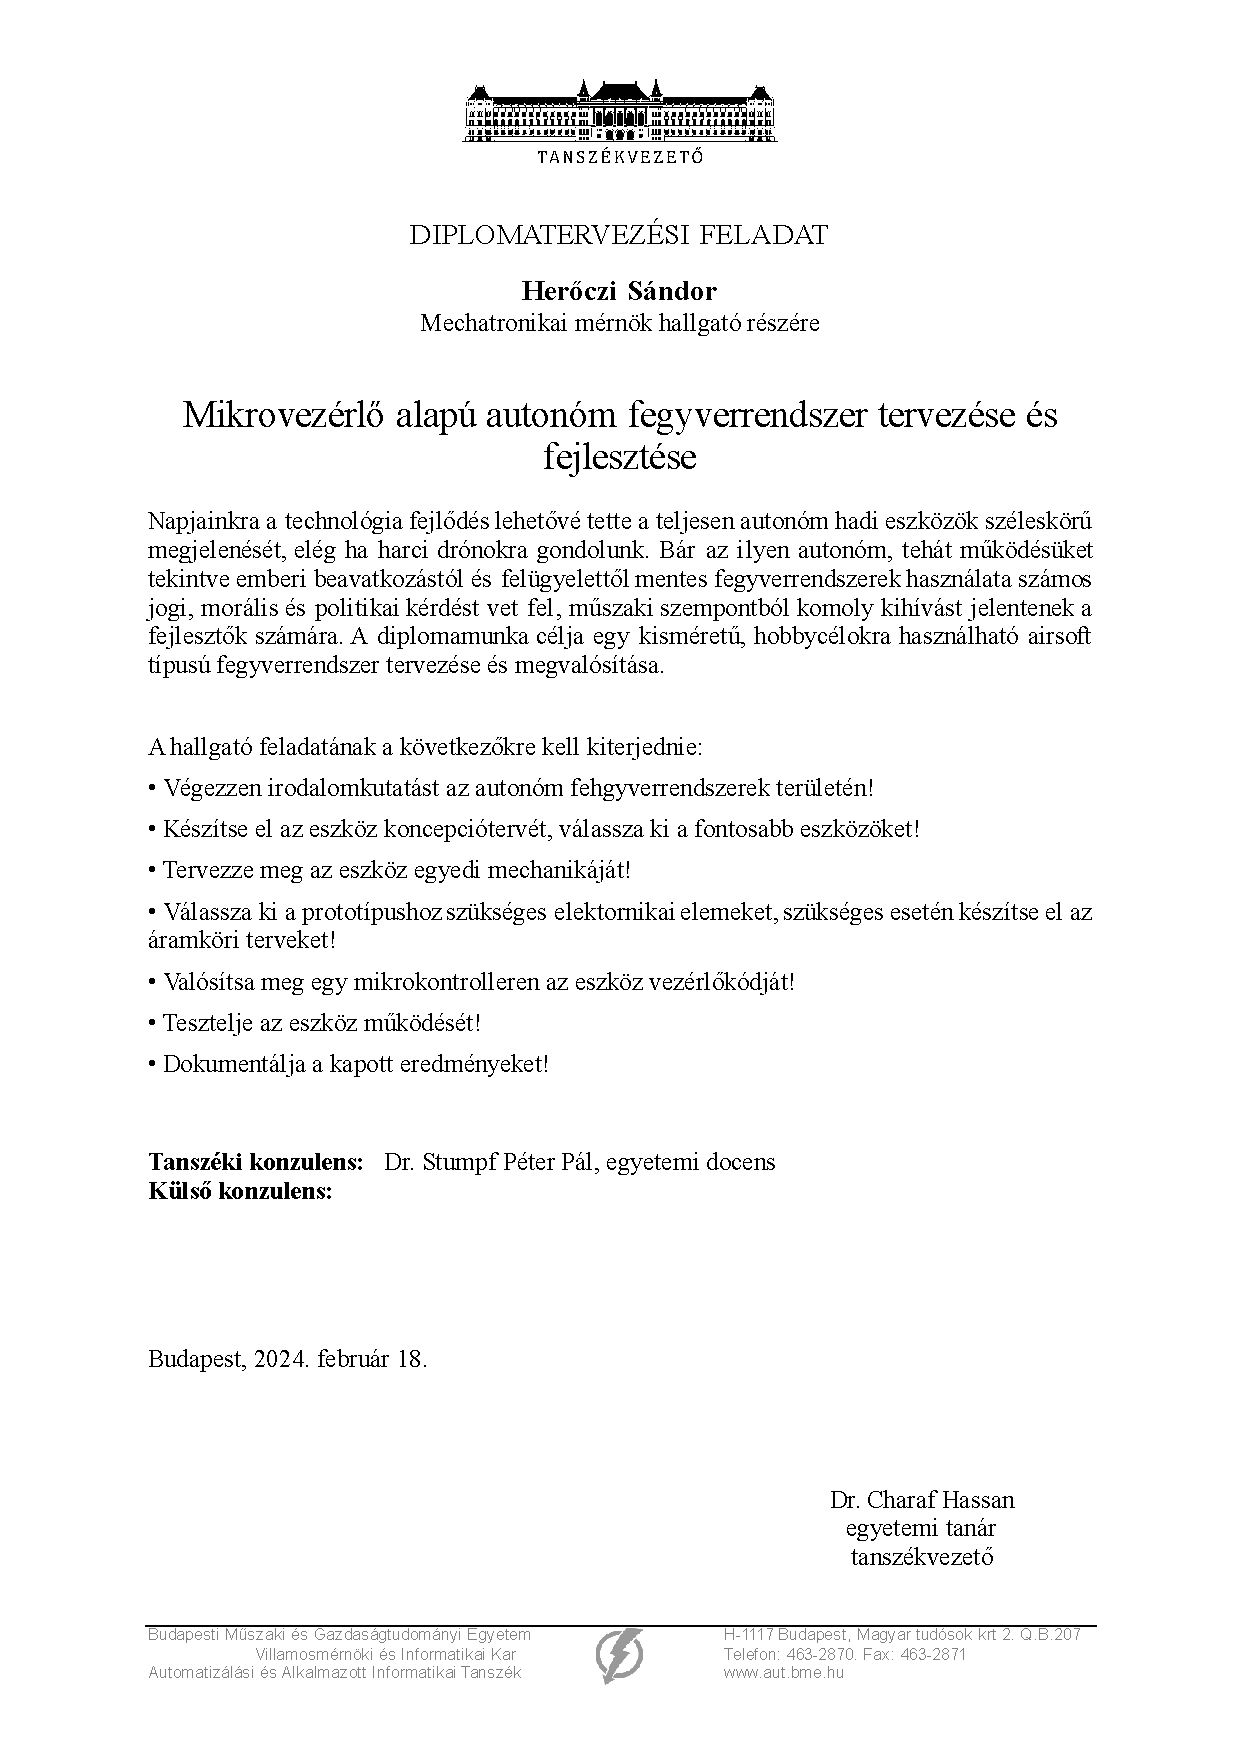
\includepdf[pages=-]{feladatkiiras.pdf}

\begin{titlepage}
	\begin{adjustwidth}{-2.5cm}{-2.5cm}

	
	\thispagestyle{empty}
	\centering

	\Large
	\rule{16cm}{1pt}\\
	\textsc{
		Budapesti Műszaki és Gazdaságtudományi Egyetem\\
		Villamosmérnöki és Informatikai Kar\\
		Automatizálási és Alkalmazott Informatikai Tanszék}\\[-0.3cm]
	\rule{16cm}{1pt}
	\end{adjustwidth}
	
	\vspace{2cm}
	
	\flushleft
	\Huge
	\textbf{\TITLE}
	
	\vspace{3cm}
	
	\Large
	\textbf{\AUTHOR}\\
	\NEPTUN\\
	
	\begin{tikzpicture}[overlay, remember picture]
		\node[anchor=center, xshift=5cm, yshift=-10cm] at (current page.center)
		{
\includegraphics[height=2cm]{autlogo}}; 
	\end{tikzpicture}
\end{titlepage}

\pagebreak

\section*{Hallgatói nyilatkozat}

Alulírott Herőczi Sándor, szigorló hallgató kijelentem, hogy ezt a diplomatervet meg nem engedett segítség nélkül, saját magam készítettem, csak a megadott forrásokat (szakirodalom, eszközök stb.) használtam fel. Minden olyan részt, melyet szó szerint, vagy azonos értelemben, de átfogalmazva más forrásból átvettem, egyértelműen, a forrás megadásával megjelöltem.\\

Hozzájárulok, hogy a jelen munkám alapadatait (szerző(k), cím, angol és magyar nyelvű tartalmi kivonat, készítés éve, konzulens(ek) neve) a BME VIK nyilvánosan hozzáférhető elektronikus formában, a munka teljes szövegét pedig az egyetem belső hálózatán keresztül (vagy hitelesített felhasználók számára) közzétegye. Kijelentem, hogy a benyújtott munka és annak elektronikus verziója megegyezik. Dékáni engedéllyel titkosított diplomatervek esetén a dolgozat szövege csak 3 év eltelte után válik hozzáférhetővé.\\

Kelt: \LOCATION, 2024.06.02.\\

\hfill
\begin{tabular}{c}
	........................................... \\
	Herőczi Sándor \\
\end{tabular}

\pagebreak

\section*{Összefoglaló}
A diplomamunkám célja egy autonóm fegyverrendszer fejlesztése és elkészítése, amely funkciójában hasonlít a valós, éles helyzetben alkalmazott rendszerekhez. Ez annyit takar, hogy a fegyvernek képesnek kell egy bizonyos méretű területet belátni, ebben felismerni és azonosítani a célpontokat, majd tüzelni, vagy engedélyt kérni tüzelésre. Ezentúl szükséges funkciója a manuális vezérlés, amely segítségével az operátor valós időben tudja távolról irányítani az eszközt, egy asztali számítógép segítségével.\\

Az eszköz alkatrészei 3D nyomtatási technológiával készültek, a kötőelemeket, csapágyakat és elektronikai elemeket kivéve, első feladatom ezek nyomtatáshelyes megtervezése volt. A következő lépés a hardver és elektronikai rendszer tervezése volt, majd a szükséges modulok, szenzorok, mikrovezérlő kiválasztása és megrendelése. Az utolsó alfeladat pedig a szoftver fejlesztése, amely jelentette mind a beágyazott vezérlő szoftvert, és a számítógépen futó felhasználói felületet is.\\

A projekt megvalósítása során végig sok időt emésztett fel a rendszer tesztelése, amelyet párhuzamosan kellett végezni a későbbi alfeladatok tervezésével. Kihívást jelentett a megfelelően részletes szakirodalom felkutatása is, ugyanis a valós megoldások paramétereit gyakran nem teszik elérhetővé civilek számára, illetve a jelenleg folyó fejlesztések is titkosítottak.\\

Úgy gondolom, a téma interdiszciplináris jellegét tekintve jól illik a mechatronikai tanulmányaiba, ugyanis egyaránt érinti a műszaki mechanika,  a gyártástechnológia, a szoftverkészítés és a jelfeldolgozás területeit.\\

Diplomamunkám eredményeként megvalósítok egy működő prototípust, amit előadás keretében fogok bemutatni. Végül pedig kitérek az esetleges hibákra amiket elkövettem, a tanulságokra és a továbbfejlesztési lehetőségekre.

\pagebreak

\section*{Abstract}
The aim of my thesis is to develop and build an autonomous weapon system that functions similarly to real-world systems used in live scenarios. This means that the weapon must be able to monitor a designated area, recognize and identify targets, then fire or request permission to fire. Additionally, a necessary feature is manual control, allowing the operator to remotely control the device in real-time using a desktop computer.\\

The components of the device were created using 3D printing technology, except for the fasteners, bearings, and electronic elements. My first task was to design these components to be suitable for printing. The next step was to design the hardware and electronic system, followed by selecting and ordering the necessary modules, sensors, and microcontroller. The final subtask was the development of the software, which included both the embedded controller software and the user interface running on a computer.\\

Throughout the project, significant time was consumed by system testing, which had to be carried out simultaneously with the planning of subsequent subtasks. A challenge was also posed by finding sufficiently detailed technical literature, as the parameters of real-world solutions are often not made available to civilians, and current developments are often classified.\\

I believe that the interdisciplinary nature of this topic fits well with my mechatronics studies, as it encompasses areas such as mechanical engineering, manufacturing technology, software development, and signal processing.\\

As a result of my thesis, I will produce a working prototype, which I will present during my final defense. Lastly, I will address any mistakes I made, lessons learned, and possibilities for future development.
\pagebreak

\tableofcontents

\pagebreak

\section{Bevezetés}

\subsection{Motiváció és háttér}

\lettrine{E}zt a projektet nem a tanszéki diplomamunkatémák listáján találtam, hanem én kerestem hozzá konzulest. Szeretném ezért először megemlíteni a személyes motivációmat, és érdekeltségeimet vele kapcsolatban. Mint a legtöbb reál beállítottságú fiú, engem is fiatal korom óta érdekel a technológia, a járművek, a gépek, vagy a fegyverek. Ezek közös metszéspontja a haditechnológia, ami általában jóval fejlettebb, mint amivel a civil életben találkozhatunk. Ez az érdeklődés megmaradt kamaszkoromra is, amikor a videojátékok által új ingerként értek a \textsl{Team Fortress 2}-ben és a \textsl{Portal}-ban lévő ún. \textbf{Sentry Gun}-ok. Ezek olyan lövegek , amelyek a lábukon állva képesek voltak forogni, és ha az ellenség a látóterükbe jutott, akkor arra tüzet nyitottak. Nyilván játékokról van szó, tehát mindig azt hittem hogy ez csak a jövő technológiája, de nem sokkal később rá kellett jönnöm, hogy nagyon is valódiak. Ezután, mikor már egyetemre jártunk, egy barátommal egyre komolyabban kezdtünk beszélgetni arról, hogy esetleg mi is tudnánk egyet építeni. Végül az egyetemi éveim végére érve el is jött a tökéletes alkalom, hogy megvalósítsam régi álmomat. \\

A szentimentalitást félretéve, természetesen nem választottam volna ezt a témát, ha nem lenne a tanulmányaim szempontjából is releváns. Úgy gondolom, ez a projekt a mechatronika oktatás sok fontos elemét magában hordozza. A feladat a mechanikai konstrukcióval kezdődik és a CAD modellezéssel, amely a gépészeti oldalát hasznosítja a képzésünknek. Foglakozni kell a hardverrel, amihez elektronikai ismeretek szükségesek. Végül pedig a szoftvert kell lefejleszteni, ami informatikai szempontból érdekes. Ráadásul az egész beágyazott környezetben történik, ami miatt még relevánsabb az \textsl{intelligens beágyazott rendszerek} specializációmhoz. Véleményem szerint a projekt nehézsége és kihívása nem az egyes alfeladatokban rejlik, hanem az egész rendszer integrálásában, egymáshoz illesztésében. \\

Szintén fontosnak tartom megemlíteni, hogy a feladat lehetőséget ad megismerni és használni pár igen modern technológiát. A közelmúltban elérhetővé (és megfizethetővé) váltak civil felhasználásra a 3D nyomtatók, valamint a fejlődés a \textsl{Deep Learning} algoritmusok terén nagyban befolyásolta a gépi látás szakterületét is. Többek között a célom, hogy jobban megismerkedjek ezekkel a módszerekkel, és alkalmazzam őket.

\pagebreak

Mint manapság az ipar minden területén, így a fegyveriparban is egyre nagyobb mértékű a digitalizáció és az automatizáció. Ennek ékes példája a távolról irányítható lőállások térnyerése, amelyeknek nagy előnye a fegyver és a tüzér egymástól való elkülönítése, aminek több előnye is van. Természetesen a legfontosabb és leginkább szembetűnő, hogy ezzel a módszerrel minimalizálható, vagy akár megszüntethető a saját embereink életének kockáztatása. Ezentúl olyan helyen is tudjuk használni ezeket az eszközöket, ahova egy tradicionális géppuskafészek telepítése nehézkes lenne, például mostoha természeti körülmények közé, egy torony tetejére, vagy akár egy hadihajó oldalára. Szintén egy nagy előny, hogy ezek az eszközök felszerelhetők több kezeléssegítő alegységgel, például hőkamerával vagy éjjellátóval. Majdnem minden, számottevő hadsereggel rendelkező országnak van saját fejlesztésű távirányított fegyverrendszere.\\


\begin{wrapfigure}{r}{0.45\textwidth}
	\centering
	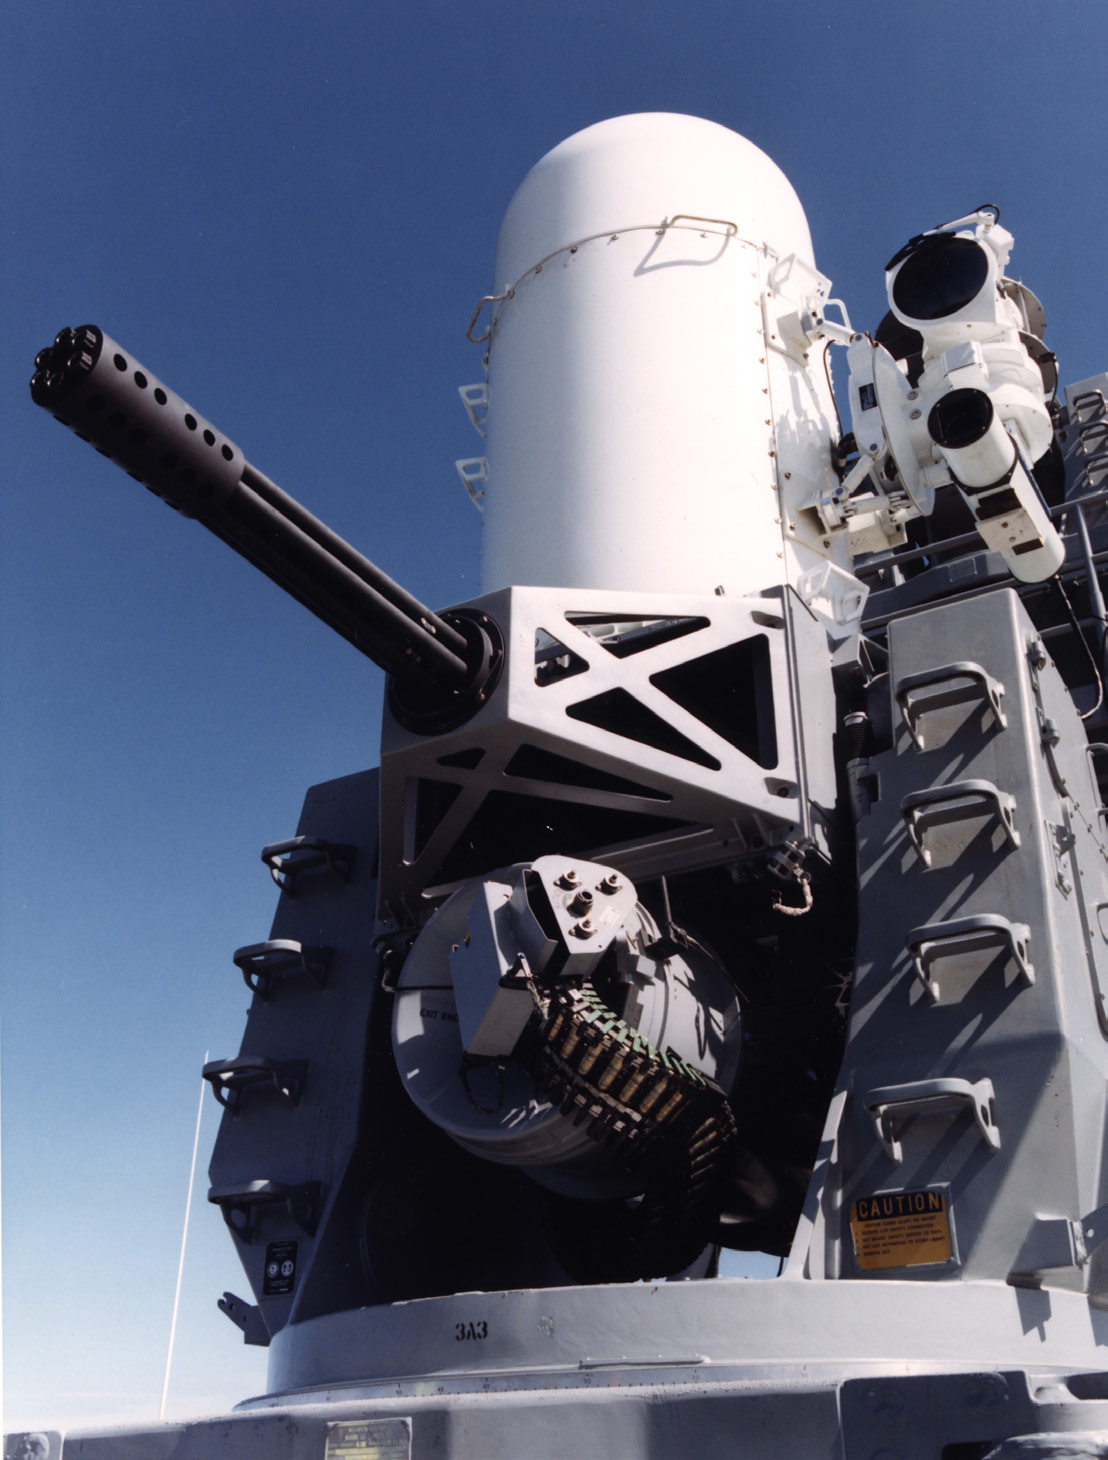
\includegraphics[width=0.95\linewidth]{irod_phalanx} 
	\caption{Phalanx CIWS rendszer}
	\label{fig:irod_phalanx}
\end{wrapfigure}

A következő lépés az automatizálás. Hiszen egyre erősebb hardverekkel rendelkezünk, egyre jobb algoritmusokat tudunk implementálni, és elértük az a szintet, hogy bizonyos helyzetekben a "gép" jobb munkát tud végezni, mint egy ember. Az első automatikus célzórendszerrel rendelkező légvédelmi gépágyú az amerikai \textsl{Phalanx CIWS} az 1970-es években került kifejlesztésre, ezzel megszületett a "Lethal autonomous weapon (LAW)" kifejezés.\\

A technológiát érthető módon leggyakrabban védelmi célokra használják, sokszor légvédelemre. A gyakorlatban nagy szerepe van Dél-Korea és Izrael védelmében, ahol a rakétatámadások mindennapos veszélyt jelentenek. Offenzív célokra a gyakorlatban még csak rakéták célzására használnak automatikát, a "terminátor" jellegű gyilkos robotok még csak fejlesztési fázisban vannak.
\pagebreak 

\subsection{Kihívások és célkitűzések}

A hagyományos, ember által irányított biztonsági rendszerek, illetve manuálisan vezérelt fegyverek hatékonysága korlátozott. Az ember reakcióideje lassú lehet krízishelyzetben, különösen ha nagy sebességű, gyors reagálású, esetleg automatizált a célpont. További gyengesége az embernek, hogy hajlamos hibázni. A fáradtság, stressz, éhség, és rengeteg egyéb tényező kényszerítheti hibára. Ez szükségessé teszi egy olyan automata rendszer kifejlesztését, amely képes azonnal reagálni, felismerni a fenyegetéseket és pontosan célozni.\\

Az automatikus gépágyúk fejlesztése során számos technikai kihívás merül fel:

\begin{list}{}{}
	\item \textbf{Célpontok felismerése és követése:} A gépágyúnak gyorsan és pontosan kell érzékelnie és nyomon követnie mozgó célpontokat. Ez kihívást jelenthet változó fényviszonyok, mozgássebességek és környezeti zavaró tényezők mellett. A gépágyúnak gyorsan és pontosan kell érzékelnie és nyomon követnie mozgó célpontokat. Ez kihívást jelenthet változó fényviszonyok, mozgássebességek és környezeti zavaró tényezők mellett. \\
	\item \textbf{Pontosság és reakcióidő:} A rendszernek gyorsan kell döntéseket hoznia, ugyanakkor elengedhetetlen a pontos célzás. A mechanikai mozgásvezérlés, a számítógépes látás és az elektronikai rendszerek szinkronizációja mind kritikus tényező a rendszer hatékonysága szempontjából. \\
	\item \textbf{Környezetérzékenység:} Külső környezeti tényezők (pl. időjárás, akadályok, fényviszonyok) befolyásolhatják a rendszer működését, ezért a szoftvernek és a hardvernek rugalmasnak és robusztusnak kell lennie. 
\end{list}
A dolgozatom célja egy innovatív megoldás kidolgozása, amely eleget tesz a megszabott követelményeknek és megoldást nyújt a fenti problémákra. \\

\pagebreak

Kiemelt célok:
\begin{list}{}{}
	\item Egy megbízható célpontfelismerési rendszer fejlesztése, amely változó környezeti feltételek mellett is képes hatékonyan működni.
	\item Egy stabil és erős mechanikai konstrukció tervezése, amely képes képes követni a szoftver utasításait.
	\item Egy olyan valós idejű szoftvervezérlési rendszer megalkotása, amely gyorsan reagál a célpontok mozgására és változására.
\end{list}

Összegezve \textbf{Egy olyan automata gépágyú fejlesztése és megépítése, amely magabiztosan képes felismerni egy célpontot, követni azt, célozni, és tüzelni.}

\subsection{Korlátozások}

Természetesen tisztában kell lenni bizonyos korlátozásokkal a projekt elkészítése közben. Két félévem van lefejleszteni az eszközt a nulláról, egyedül vagyok, és nincsen százmilliós büdzsém, mint az iparban hasonló kutatással foglalkozó csapatoknak. Ebből kifolyólag reálisan kell látni a helyzetet, és úgy meghatározni a követelményeket, hogy egy egyetemi hallgató számára is elérhető legyen. \\

A kamerarendszer például, amit a valós megoldásokban használnak, önmagában tízmilliós tétel szokott lenni. Sajnos az én megvalósításom valószínűleg nem fog működni sötétben, nagy távolságokban, vagy esőben, hiszen a költségvetésbe nem fér bele az éjjellátó, a hőkamera, az optikai zoom vagy több kamerából álló rendszer.\\

Nem áll rendelkezésemre korlátlanul se CNC gép, se fém 3D nyomtató, így a legtöbb alkatrész műanyagból kell 3D nyomtatnom. Ez befolyásolhatja a szerkezet stabilitását, amit figyelembe kell venni a későbbiekben.\\

És végül fontos megemlíteni, hogy mivel éles fegyvert alkalmazni minden bizonnyal a törvénybe ütközne, ezért valamilyen játékfegyvert kell majd használnom. Ez befolyásolni fogja a gépágyú pontosságát, amit szintén figyelembe kell venni a tervezéskor és értékeléskor.\\


\pagebreak

\subsection{Erkölcsi nyilatkozat}
Az automata fegyverrendszer morális megítélése vitatott téma, ezért szeretném kijelenteni, hogy diplomamunkám, melynek címe \textsl{„Mikrovezérlő alapú autonóm fegyverrendszer tervezése és fejlesztése”}, kizárólag tanulányni és mérnöki célokat szolgál. A dolgozatom keretében fejlesztett prototípus semmilyen formában nem szándékozik vagy ösztönzi az erőszakos, káros vagy törvénysértő tevékenységeket. Fejlesztésem célja a technológiai kutatás, a mechatronikai és automatizálási rendszerek megismerése, illetve a gépi látás alkalmazásainak tanulmányozása. \\

Határozottan elhatárolódom bármilyen rosszindulatú felhasználástól, és hangsúlyozom, hogy a projekt eredményei nem használhatók fel ártalmas vagy illegális célokra. A munka során mindvégig tiszteletben tartottam az etikai irányelveket, és felelős mérnöki magatartást tanúsítottam. Az általam fejlesztett rendszer kizárólag oktatási, kutatási és technológiai demonstráció célját szolgálja.

\pagebreak


\section{Irodalomkutatás}
A legjelentősebb katonai hatalmak mindegyike rendelkezik távvezérelt fegyverrendszerekkel, leggyakrabban valamilyen távolról irányított gépfegyver formájában. Azonban se az egyes országok nemzetbiztonságának, se a fegyveripari partnercégeknek nem áll érdekében a szükségesnél több információt kiadni. Ez egy kicsit megnehezítette az irodalomkutatást, de a képek alapján azért sok információt ki lehet nyerni.

\subsection{Megvalósult rendszerek} \label{sec:valos}

\paragraph{CROWS \cite{crows}}
Az egyik legnagyobb darabszámban gyártott távirányított fegyverrendszer az amerikai \textsl{CROWS} rendszer, amely a NATO-országokban, köztük Magyarországon is rendszeresített. Ennek értelmében telepíthető sok NATO által használt páncélozott járműre, köztük a Humvee-ra, a Stryker-re, és a Buffalo MRAP-re. Több verziója létezik több kaliberrel, a \ref{fig:irod_crows}. ábrán egy M240B géppuskával látható.\\

\begin{figure}[h!]
	\centering
	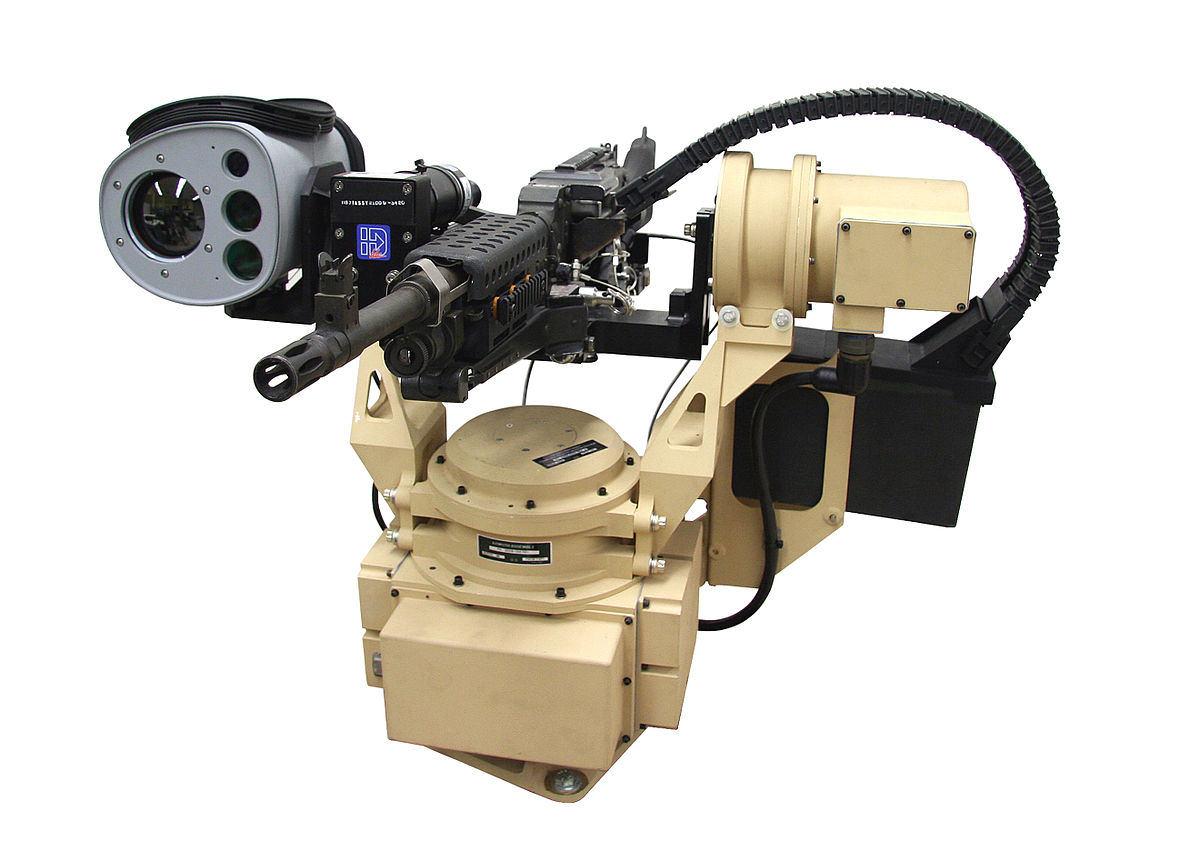
\includegraphics[width=1\linewidth]{irod_crows}
	\caption{Az amerikai CROWS rendszer}
	\label{fig:irod_crows}
\end{figure}

A szerelék a fegyverrel együtt $360^\circ$-ban képes elfordulni, és $-20^{\circ}$-tól $+60^{\circ}$-ig tud billenni. A fegyvercső giroszkóppal stabilizált. A kezelő egy 15 hüvelykes kijelzőn tud célozni a fegyverrel. A rendszer a sima kamera mellett rendelkezik hőkamerával is, így éjszaka is használható. Mind a két kamera el van látva lézeres távolságmérővel, amivel rá lehet állni a célpontra, és a jármű mozgása közben is lehet azt követni. A kamerát és a fegyvert lehet külön is mozgatni, ami azért hasznos, mert anélkül lehet követni a gyanús alakok mozgását, hogy félelmet keltenénk az emberekben.

\paragraph{Arbalet-DM \cite{arbalet}}
A \textsl{CROWS} rendszer orosz megfelelője a hasonló kialakítású \textsl{Arbalet-DM} (\ref{fig:irod_arbalet}.ábra). Ennek a rendszernek az alapja a 12.7 mm-es KORD nehézgéppuska. Rendelkezik 4 gránátvetővel is, amelyek füstfüggöny felhúzására használható. A kamera és a fegyver elhelyezése, de még a lőszer pozíciója is teljesen hasonló az amerikai párjához.

\begin{figure}[h!]
	\centering
	\includegraphics[width=1\linewidth]{irod_arbalet}
	\caption{Az orosz Arbalet-DM rendszer}
	\label{fig:irod_arbalet}
\end{figure}

A rendszer $360^\circ$-ban képes elfordulni, és $-20^{\circ}$-tól $+70^{\circ}$-ig tud billenni, tehát egy kicsit nagyobb részt tud lefedni, mint a CROWS. A hatótáv nappal 2000 m, éjszaka 1500 m. Ez a rendszer is el van látva hőkamerával és lézeres távolságmérővel.

\paragraph{DeFNder \cite{defnder}}
A következő megoldás a belga \textsl{DeFNder} termékcsalád, amelynek két tagja a \textsl{Light} és a \textsl{Medium}(\ref{fig:irod_defnder}. ábra). Értelem szerűen kettő közül az utóbbi az, amelyre nehezebb fegyverzetet lehet telepíteni. A függőleges tengelyen $360^\circ$-ban képes elfordulni 90 fok/másodperc sebességgel, a vízszintes tengelyen $-45^{\circ}$-tól $+75^{\circ}$-ig tud billenni, 60 fok/másodperc sebességgel. Opcionálisan ellátható infravörös- és hőkamerával a rossz látási körülmények esetére, valamint lézeres távolságmérővel a ballisztikai kompenzációhoz.
\begin{figure}[h!]
	\centering
	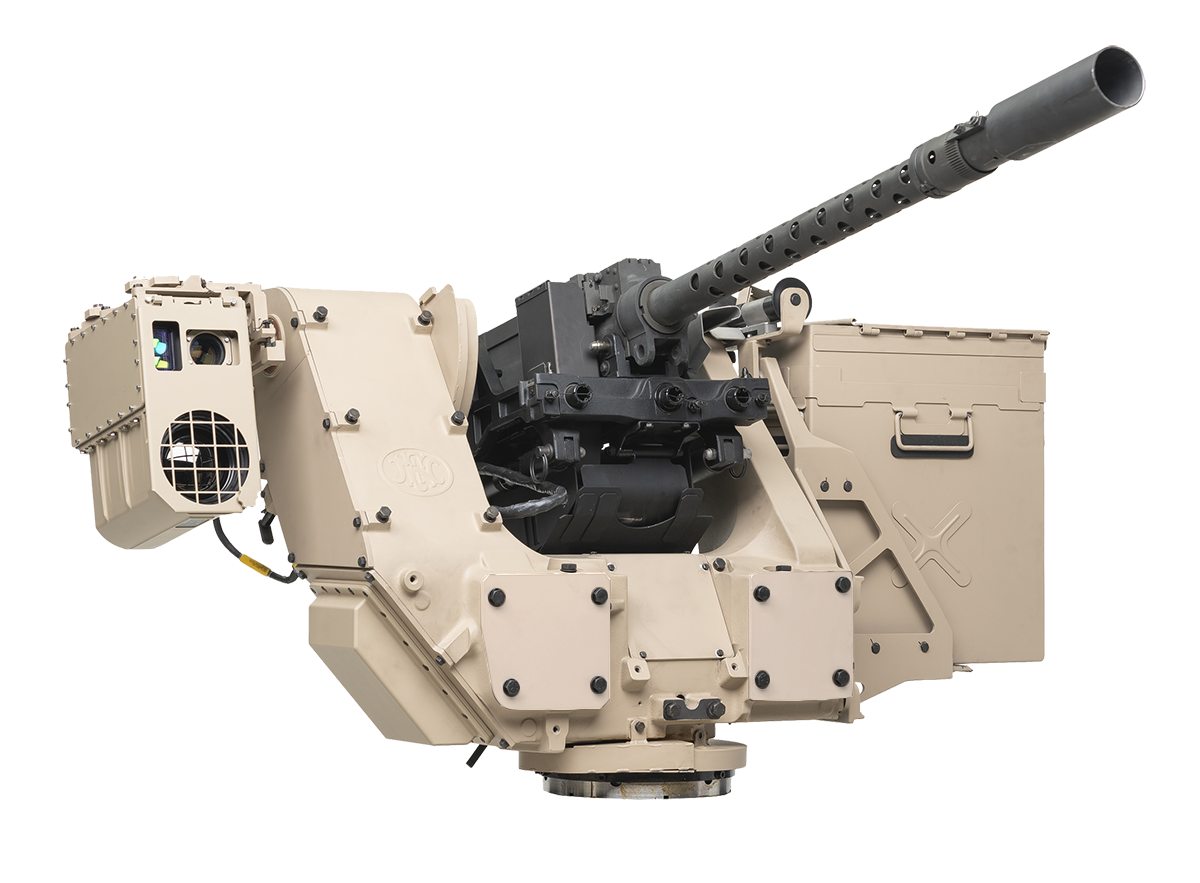
\includegraphics[width=1\linewidth]{irod_defnder}
	\caption{A belga DeFNder rendszer}
	\label{fig:irod_defnder}
\end{figure}

Elég sok közös vonást találtam a fentebb említett rendszerekben. Az elrendezésük nagyon hasonló, van egy függőleges forgástengely nagyjából a teljes rendszer súlypontján keresztül, valamint egy vízszintes forgástengely, nagyjából a fegyver csövével egy síkban. Erre valószínűleg azért van szükség, hogy a tüzelés során keletkező erők ne ébresszenek csavarónyomatékot a mozgató mechanizmuson. Az én esetemben nagy erők nem fognak ébredni, de a tervezési elvet érdemes követni.

\paragraph{Samsung SGR-A1}
Az egyetlen, valós harci helyzetben használt, teljesen autonóm gépágyú a koreai fejlesztésű \textsl{Samsung SGR-A1}. A két Korea között húzódó demilitarizált övezet (DMZ) egy 250 km hosszú, 4 km széles sáv, amelyet mind a két oldalon szigorúan ellenőriznek. A határ folyamatos felügyelete rengeteg ember munkájába kerül, ami egy demográfiai válságban lévő ország csökkenő hadseregében egyre értékesebb. Főleg annak tekintetében, hogy csupán járőrözni és figyelni a határt nem feltétlenül igényli egy ember jelenlétét. Ennek tudatában fejlesztették ki a Samsung és a Korea Egyetem mérnökei az SGR-A1 fegyverrendszert. Hőkamerával és éjjellátóval felszerelve napközben 4 km-ről, éjszaka 2 km-ről képes azonosítani potenciális célpontokat, tehát tulajdonképpen a DMZ teljes szélességében. Képes felismerni az embereket, követni őket, és megkülönböztetni az állatoktól. Hangfelismeréssel képes azonosítani a közeledő személyeket: amennyiben valaki 10 m-nél közelebb kerül és nem azonosítja magát, a rendszer riaszthat, gumilövedéket lőhet, vagy használhatja a K-3 gépfegyverét.

\begin{figure}[h!]
	\centering
	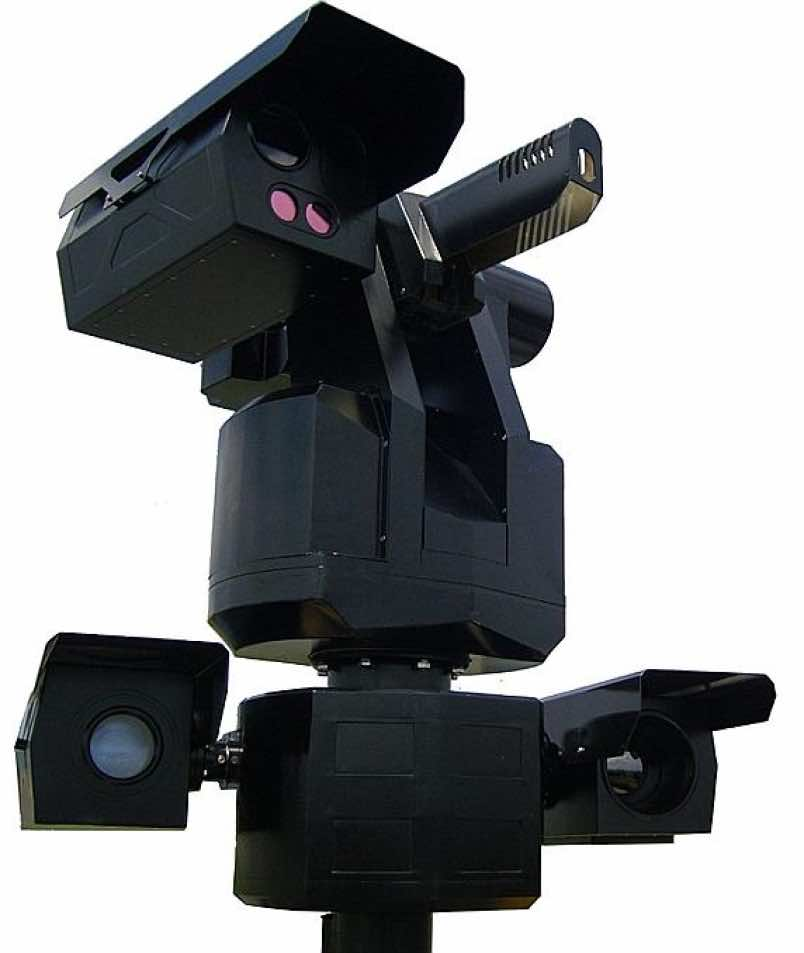
\includegraphics[width=0.5\linewidth]{irod_samsung}
	\caption{Samsung SGR-A1}
	\label{fig:irod_samsung}
\end{figure}

Sok szakértő találgatja, hogy a rendszer lőhet-e emberi engedély nélkül, és a hivatalos koreai álláspont az, hogy nem. Azonban ha már bemérte és ellenségként azonosította a célpontot, akkor nehéz elképzelni, hogy pont a ravaszt ne tudná meghúzni.

\pagebreak

\subsection{Tüzelési mechanizmus}

A korábban említett rendszerek éles fegyverekkel vannak felszerelve, ami az én esetemben sajnos nem megvalósítható. Így valamilyen más megoldást kellett találni, ami legális, és megfelelően be lehet vele mutatni a célfelismerés és célzás működését. 


\paragraph{Paintball}

Több, a diplomamunkámhoz hasonló projektet is találtam, amelyek paintball puskákat használnak. Ezek a puskák sűrített levegőt alkalmaznak, hogy egy festékkel töltött golyót lőjenek ki. A torkolati sebességük nagyjából 280 fps, maximális hatékony távolságuk kb 25-30 m. Mivel a lövedék alakja gömb, és a cső sincs huzagolva, ezért nem túl pontos, főleg hosszú távon.\\

\begin{figure}[h!]
	\centering
	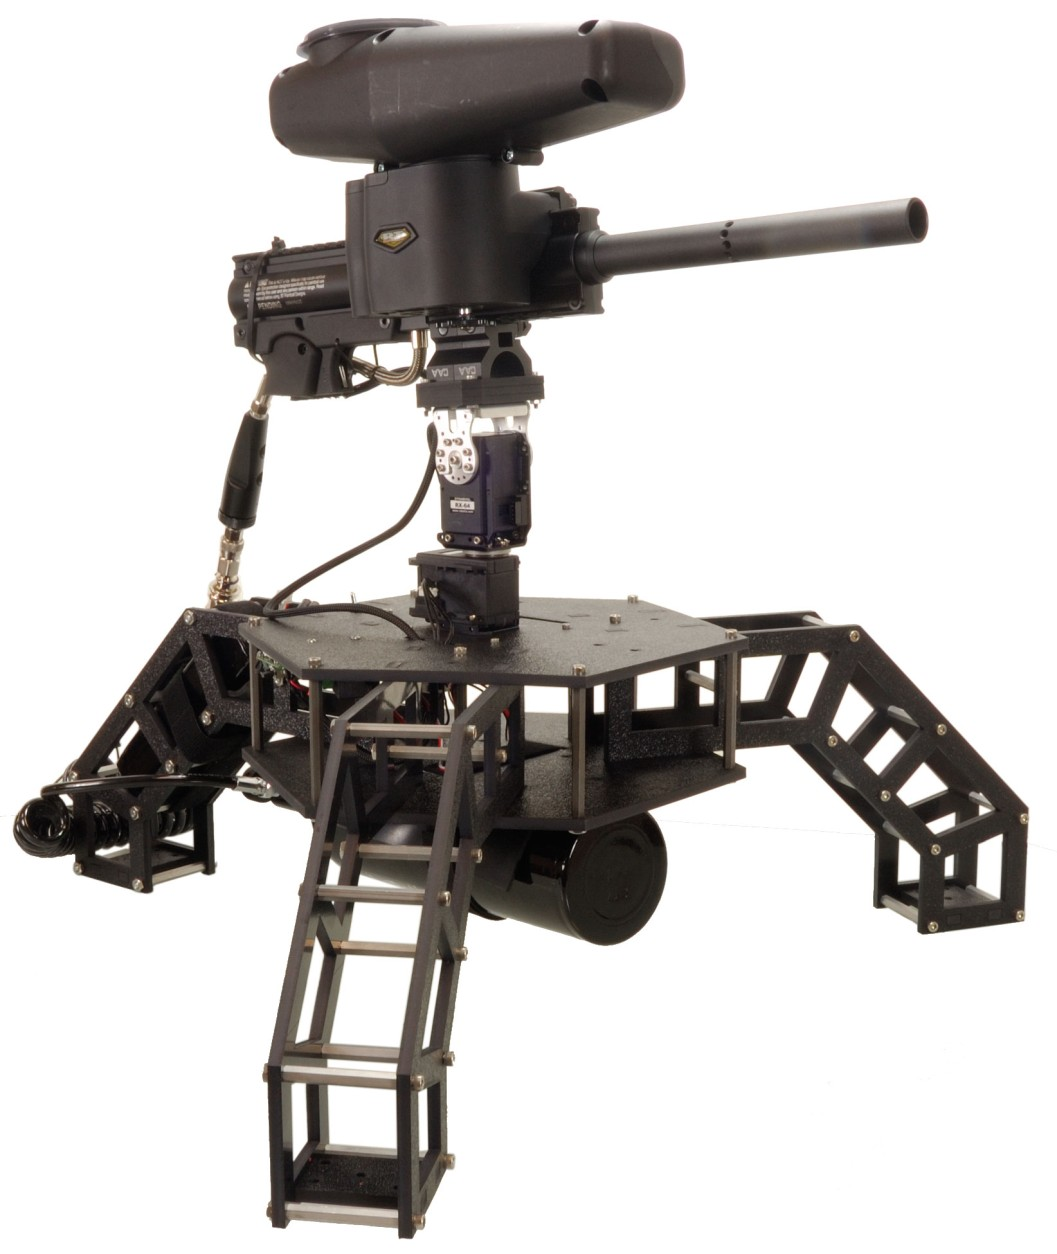
\includegraphics[width=0.6\linewidth]{irod_paintball}
	\caption{Paintball puska alapú rendszer}
	\label{fig:irod_paintball}
\end{figure}

További problémák, hogy a legolcsóbb paintball puska is 70000 Ft. fölött van, valamint a lövedék is viszonylag drága, és nem lehet újrahasznosítani. Ezentúl a fegyverek nagyok, nehezek, és ezért nehéz a beépítésük. 


\paragraph{Nerf}

A Nerf fegyverek a legelterjedtebb játékfegyverek. Sűrített levegővel lőnek ki egy hosszúkás szivacs lövedéket. A sűrített levegőt egy megfeszített rugó elengedésével érik el, amelyet vagy kézzel, vagy valamilyen áttételes villanymotorral húznak fel. A legjobb modellek torkolati sebessége 70 fps körül van, és kb. 15 m a hatótávolságuk. Ezen a távon viszonylag pontosak a lövedék kialakításából adódóan, de jelentős az esés, így a ballisztikai pályát komolyan kell venni. \\

Ezek a fegyverek modelltől függően 10000 Ft. - 40000 Ft. között mozognak, de a lövedékeket újra lehet használni. Az a probléma itt is fennáll, hogy nagy a fegyver teste, így nehezebb beépíteni. 

\paragraph{Airsoft}

Az airsoft fegyverek hasonló módon működnek, mint a Nerf puskák, de egy kisebb, műanyag golyót lőnek. Az elektromos airsoft fegyverek torkolati sebessége általában 300 fps és 400 fps között van, ami befolyásol a golyók tömege, a rugó minősége és rengeteg egyéb alkatrész. A hatótávjuk az átlagos fegyvereknek kb. 50 m, de fejlesztésekkel elérheti a 90 m-t is. A lövedék itt is golyó és a cső sincs huzagolva, mint a paintballnál, azonban az airsoft esetében használnak ún. hop-up kamrákat, amelyek perdületet adnak a golyónak.\\

Az airsoft fegyverek legnagyobb előnye a többi lehetőséggel szemben, hogy van egy kompakt egység, a "gearbox", ami felelős az elsütésért. Ezt ki lehet szedni egy fegyverből, vagy akár külön is meg lehet venni. Ez okkal nagyobb szabadságot ad a beépítéshez, és a végeredmény is sokkal kompaktabb lesz. Az elsütés is csak az áramkör zárását jelenti a gearboxban, ami egyszerűen vezérelhető a mikrokontrollerrel.
\pagebreak

\section{Rendszertervezés és követelmények}
\subsection{Rendszeráttekintés}
Az autonóm fegyverrendszer fejlesztése során egy komplex mechatronikai rendszert kellett megvalósítani, amely több különálló modul együttműködését biztosítja. A rendszer fő komponensei közé tartozik a mechanikai szerkezet, az elektronikai hardver, az érzékelők, a vezérlő egység, valamint a szoftveres háttér. Ezek együttesen biztosítják a rendszer autonóm és manuális működését. Az alábbiakban részletes áttekintést adok a rendszer főbb elemeiről és azok feladatáról.

\subsubsection*{Mechanikai konstrukció}

A váz gyanánt tulajdonképpen egy kéttengelyes pan-tilt mechanizmust kellett megvalósítanom, ami felelős a fegyver stabilan tartásáért és precíz mozgásáért. A váz építőelemei zömében 3D nyomtatási technológiával készültek, ami lehetővé tette a problémák gyors kiküszöbölését, illetve a nagyfokú szabadságot a tervezés során. Ahol tudtam, kereskedelemből beszerezhető alkatrészeket használtam, például a csapágyakat és a kötőelemeket.

\subsubsection*{Elektronikai rendszer}

Az elektronikai rendszer két fő eleme a Raspberry PI, illetve a gearbox volt. Mivel a gearbox igen nagy áramot képes felvenni, külön tápegységgel kellett ellátnom a mikrovezérlőt illetve a golyó kilövéséért felelős elektronikát. A motorok vezérléséért egy kereskedelemben kapható, Raspberryvel kompatibilis shieldet használtam, amely jelentősen megkönnyítette a NEMA-17 típusú léptetőmotorok csatlakoztatását. A lézer diódát és szükséges szenzorokat a Raspberry PI GPIO lábairól vezéreltem, ahogy a gearbox aktiválásáért felelős relét is. A kamera modul egy Raspberry PI Camera V2 volt, amit a mikrovezérlőn található foglalaton keresztül tudtam elérni.

\subsubsection*{Számítógépes vezérlés és szoftveres háttér}

A szoftverfejlesztés során két fő területet kellett lefedni: a vezérlőszoftvert, amely a mikrokontrolleren fut, és az asztali alkalmazást, amely a felhasználói felületet és a magas szintű irányítást biztosítja. A beágyazott vezérlő szoftver felelős a léptetőmotorok mozgatásáért, valamint a szenzorokból érkező információ feldolgozásáért. A számítógépen futó szoftver feladata a felhasználó parancsainak feldolgozása és továbbküldése, valamint a kamera képének megjelenítése valós időben. Mivel a feladat összetett, mind a PC, mind a Raspberry Pi oldaláról történik küldés és fogadás is, ezért több szálon fut egyszerre a szoftver. A két egység közötti kommunikáció során kulcsfontosságú a megfelelő sebesség, ezért a vezetékes kapcsolat mellet döntöttem.

\subsection{Követelmények}\label{sec:kov}

%A követelményeket egyrészt a később említett irodalomkutatás, másrészt pedig a saját ötleteim és a konzulensemmel való egyeztetés alapján alakítottam ki. Az "autonóm fegyverrendszer" alatt én egy olyan eszközt értek, ami egy pontban elhelyezve képes a környezetében felismerni a betanított célpontot, és arra tüzelni. Erre jó fikciós példa a \textsl{Portal} című játékban található \textsl{Sentry turret}, amely a \ref{portalsentry}. ábrán látható. Természetesen a konstrukciós tervezéshez nem ezt vettem alapul, de a működési elvhez adhat jó ötleteket akkor is, ha csak fikció. \\
%
%\begin{wrapfigure}{r}{0.45\textwidth}
%	\centering
%	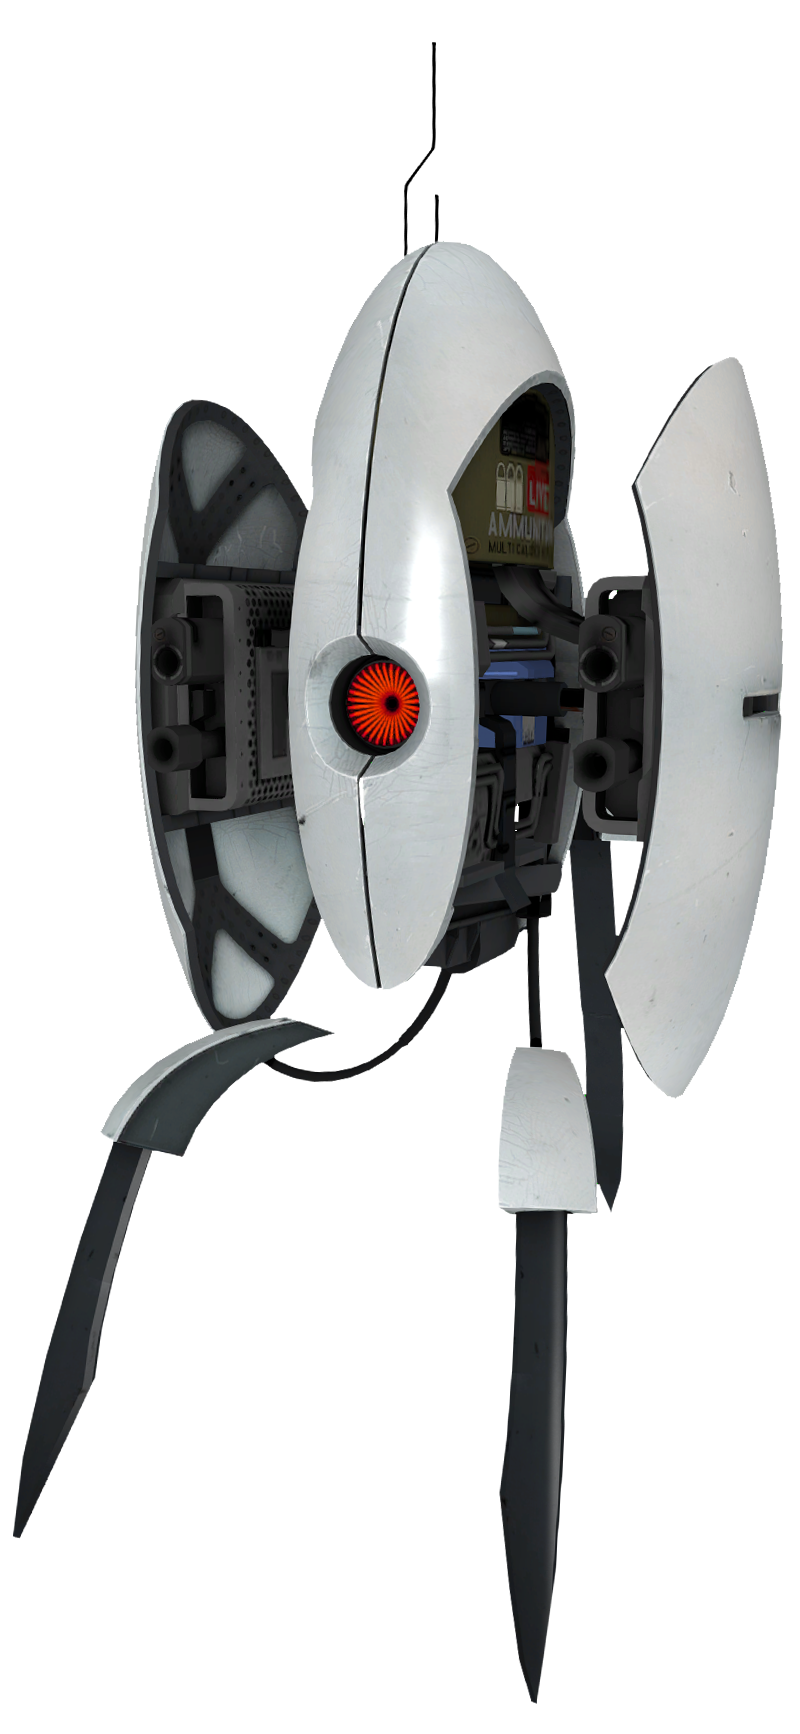
\includegraphics[width=0.8\linewidth]{portalsentry}
%	\caption{Sentry Turret}
%	\label{portalsentry}
%\end{wrapfigure}
%
%Szeretném a rendszert úgy megvalósítani, hogy a célfelismerés és tüzelést lehessen vezérelni "kézi vezérléssel", ahogy a valós katonai rendszerek többsége működik, illetve egy teljesen automatikus gépi látás algoritmussal. Automata működés során is talán az lenne a legéletszerűbb, hogy a célpont megtalálása és becélzása lenne automatikus, a tüzelés pedig emberi engedélyezést igényel, ezzel egy fokkal morálisabbá téve a projektet.\\
%
%A hatásos távolságot én 10m-ben határoztam meg. Ezen a távolságon fel kell ismernie és el kell találnia egy 30x30 cm-es célpontot. Ezentúl szeretném, ha le tudná követni a 10 km/h-val futó ember mozgását. Ezek a határértékek a konstrukció tervezésénél fontos szempontok lesznek, tehát a későbbi fejezetekben számolok velük.\\
%
%\pagebreak

Az autonóm fegyverrendszer fejlesztése során számos követelményt kellett figyelembe venni annak érdekében, hogy a rendszer megbízhatóan, hatékonyan és biztonságosan működjön. Ezek a követelmények a rendszer mechanikai, elektronikai és szoftveres elemeire egyaránt kiterjedtek. A következő szakaszokban részletezem a legfontosabb műszaki és funkcionális követelményeket.

\subsubsection*{Mechanikai követelmények} 

A mechanikai komponensek tervezése során az alábbi követelményeknek kellett megfelelni:
\begin{list}{}{}
	\item \textbf{Stabilitás és pontosság:}  A fegyverrendszer mechanikai szerkezetének stabilnak és tartósnak kell lennie annak érdekében, hogy a lövések közben ne mozduljon el, és ne veszítse el a célpontot. Ugyanakkor elegendő pontosságot kell biztosítania a célpont precíz követéséhez.
	\item \textbf{Fürgeség:} A rendszernek képesnek kell lennie a fegyver gyors és pontos mozgatására a pan-tilt mechanizmus segítségével. Ennek megfelelően a szervomotoroknak kellően gyorsnak és erősnek kell lenniük ahhoz, hogy valós időben tudják követni a mozgó célpontokat.
	\item \textbf{Strapabíró konstrukció:} Habár nagy terhelés nem fogja érni, a gearboxból jöhetnek rezgések, rángások, amik esetleg problémát jelenthetnek egy alulméretezett alkatrész esetében.
\end{list}

\subsubsection*{Elektronikai követelmények}

Az elektronikai rendszer megbízható működése érdekében az alábbi követelményeknek kellett eleget tenni:

\begin{list}{}{}
	\item \textbf{Megfelelő teljesítmény:}  A szervomotoroknak és szenzoroknak megfelelő tápegységre van szükségük, amely stabil energiaellátást biztosít. A rendszer energiaigényét előzetesen fel kellett mérni, hogy a tápegység terhelés alatt is megfelelően működjön.
	\item \textbf{Szenzorok pontossága:} A kamerának és egyéb szenzoroknak elegendő felbontással és érzékenységgel kell rendelkezniük ahhoz, hogy képesek legyenek a célpontokat megfelelően azonosítani. A valós idejű képfeldolgozás nagy adatsebességet és megbízható szenzorjeleket igényel.
	\item\textbf{ Vezérlés:} A mikrokontrollernek kellően gyorsnak kell lennie, hogy a valós idejű adatokat folyamatosan feldolgozza és a vezérlési parancsokat késlekedés nélkül végrehajtsa.
\end{list}


\subsubsection*{Szoftveres követelmények}

A rendszer működéséhez szükséges szoftverfejlesztés során a következő követelményeknek kellett megfelelni:

\begin{list}{}{}
	\item \textbf{Valós idejű feldolgozás:}  A számítógépes látás szoftverének valós időben kell elemeznie a kamerák által közvetített adatokat, felismerve a célpontokat és kiszámítva a mozgás irányát. A célzási és lövési döntések gyors és hatékony adatfeldolgozást igényelnek.
	\item \textbf{Biztonságos működés:} A rendszernek rendelkeznie kell olyan szoftveres biztonsági funkciókkal, amelyek megakadályozzák a véletlen tüzelést. Ez magában foglalja a lövési engedélykérés mechanizmusát és a manuális vészleállítás lehetőségét.
	\item \textbf{Felhasználói interfész:} Az felhasználónak egyszerű és intuitív felhasználói felületet kellett biztosítani, amelyen keresztül könnyedén vezérelheti a rendszert, illetve áttekintheti a célpontok adatait és a kamera képét. A felületnek támogatnia kell a kézi irányítást és a lövési parancsok kiadását.
\end{list}



 
\subsubsection*{Funkcionális követelmények}

A rendszer teljes funkcionalitásának biztosítása érdekében a következő kritériumoknak kellett megfelelni:

\begin{list}{}{}
	\item \textbf{Autonóm működés:} A rendszernek képesnek kell lennie arra, hogy teljesen önállóan felismerje és kövesse a célpontokat, valamint meghozza a tüzelési döntéseket az előre meghatározott paraméterek alapján.
	\item \textbf{Manuális vezérlés:} Az autonóm működés mellett manuális vezérlési lehetőséget is kellett biztosítani az operátor számára. Ezen keresztül a felhasználó közvetlenül irányíthatja a fegyvert és manuálisan adhat lövési parancsot.
\end{list}

\subsubsection*{Biztonsági követelmények}

Az autonóm fegyverrendszerek használatával kapcsolatban különösen fontos a biztonsági követelmények teljesítése:

\begin{list}{}{}
	\item \textbf{Vészleállítás:} A rendszernek rendelkeznie kell egy vészleállító gombbal, amely azonnal megszakítja a fegyver működését, ha bármilyen hiba vagy vészhelyzet lép fel.
	\item \textbf{Engedélyezési mechanizmus:} A tüzelési parancs kiadása előtt a rendszernek engedélyt kell kérnie az operátortól, ezzel minimalizálva a véletlen tüzelés kockázatát.
	\item\textbf{ Adatbiztonság:} A vezérlő szoftver és az operátor közötti kommunikáció titkosítva kell, hogy legyen, hogy megakadályozza a külső hozzáférést és a rendszer kompromittálását.
\end{list}

\subsubsection*{Környezeti követelmények}

A rendszernek különféle környezeti feltételek között is megbízhatóan kell működnie:

\begin{list}{}{}
	\item \textbf{Hőmérsékleti tűréshatár:}A rendszernek képesnek kell lennie normál működésre különböző hőmérsékleti körülmények között, amelyek tipikusan a beltéri használat során fordulnak elő.
	\item \textbf{Nedvesség és porállóság:} A rendszert úgy kell megtervezni, hogy ellenálljon a kisebb por- és nedvességterhelésnek, különösen, ha kültéri használatra is szükség van.
\end{list}

\pagebreak
\section{Mechanikai tervezés}
A mechanikai tervezést egy kinematikai modell kidolgozásával kezdtem, majd a meglévő, kereskedelemben kapható alkatrészek méreteihez igazítva megterveztem a 3D CAD modellt. Ezután finomhangoltam a 3D nyomtatási technológiához megfelelően.
\subsection{Kinematika}
A rendszer kinematikai modellje hasonlatos a biztonsági kamerákhoz, aminek elnevezése Pan-Tilt-Zoom, röviden PTZ. Ennek lényege a 360 fokban elforgatható függőleges tengely, és egy általában korlátoltabb vízszintes tengely. Előnyük, hogy nagy sebességgel tudnak irányt változtatni, és nagy területet képesek belátni. A zoom aspektus az én esetemben nem fontos, hiszen nem a kamera a fő funkció. A \ref{fig:mech_pantilt}. ábrán erről látható illusztráció.

\begin{figure}[h!]
	\centering
	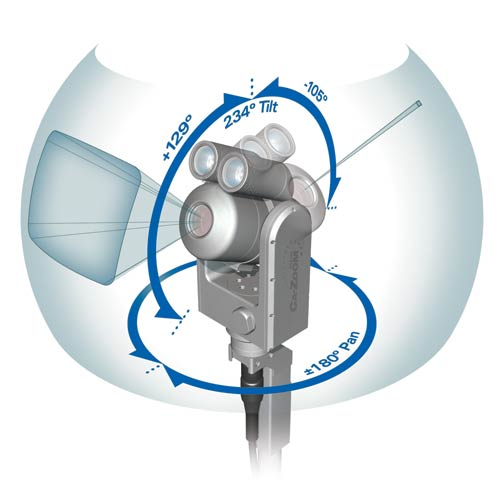
\includegraphics[width=0.6\linewidth]{mech_pantilt}
	\caption{PTZ kamera}
	\label{fig:mech_pantilt}
\end{figure}

A \ref{sec:valos}. bekezdésben vizsgált rendszerek is hasonlóképpen mozognak. Ezek közelebbi vizsgálata után elkezdtem kidolgozni a saját koncepciómat. Szemléltetésképpen készítettem a \ref{fig:megval_mockup}. ábrát. Az egyszerűség kedvéért a fegyver csövét egy síkba terveztem a pan és tilt tengelyekkel, ez megkönnyíti a későbbi számításokat.

\begin{figure}[h!]
	\centering
	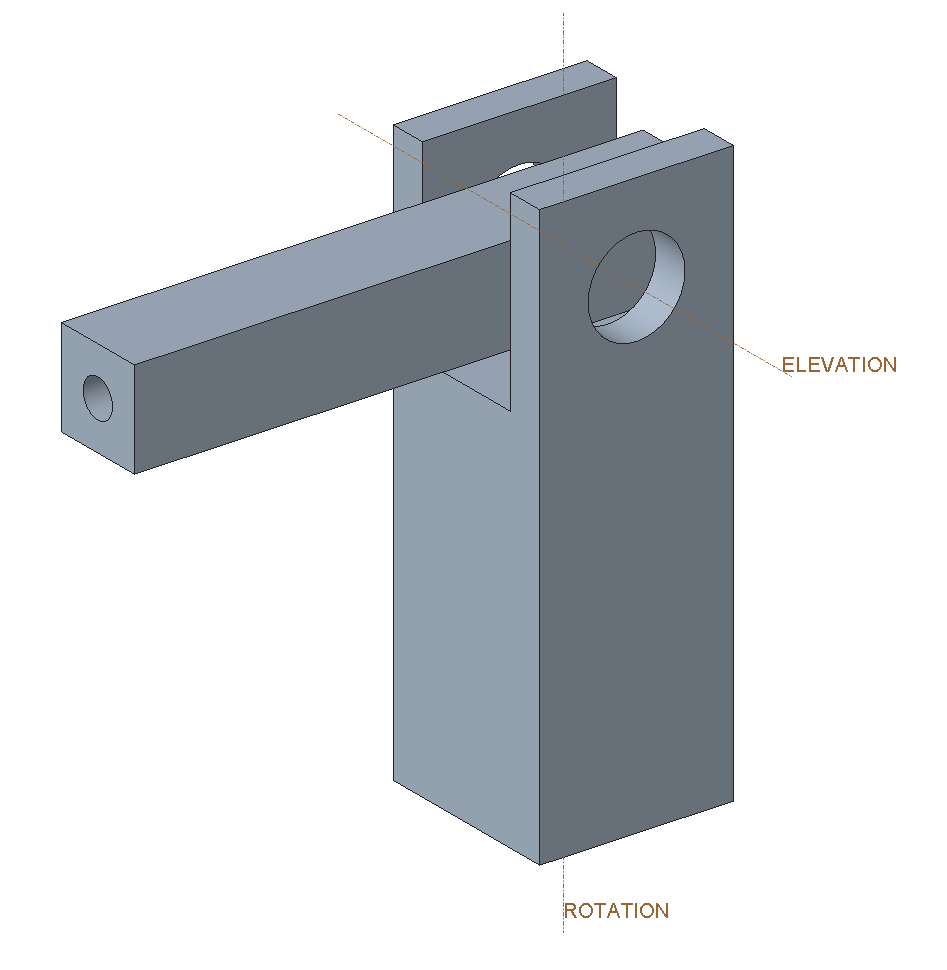
\includegraphics[width=0.6\linewidth]{mockup}
	\caption{Egyszerűsített kinematikai ábra}
	\label{fig:megval_mockup}
\end{figure}

Ki kellett számolnom bizonyos geometriai megkötéseket, amelyek szükségesek a tervezéshez, illetve az alkatrészek kiválasztásához. \\

A torony szükséges fordulatszámát a következőképpen lehet kiszámolni:


\begin{equation}
	rpm_{min} = \frac{v_t}{2 \cdot \pi \cdot r} = \frac{2.778 \w{m/s}}{2 \cdot \pi \cdot \w{m}} = 0.442 \w{1/s} = 26.526 \w{1/min}
\end{equation}

ahol:

\begin{tabular}{cl}
	$v_t$ & A célpont sebessége a fegyvercsőre merőlegesen, \\
	$r$ & A távolság a célpont és a rendszer között\\
\end{tabular}

Meg lehet állapítani a torony mozgásának felbontását is, tehát hogy hány fokonként lehet állítani a mozgását.

\begin{equation}
	\alpha_{min} = \arcsin\left(\frac{a}{2 \cdot r}\right) \cdot 2 = \arcsin\left(\frac{0.3 \w{m}}{2 \cdot 10 \w{m}}\right) \cdot 2 = 1.719 {^\circ}
\end{equation}

ahol:

\begin{tabular}{cl}
	$a$ & A célpont mérete  \\
	$r$ & A távolság a célpont és a rendszer között\\
\end{tabular}
\pagebreak
\subsection{Mechanikai alkatrészek}
\subsubsection*{Elsütő mechanizmus}
Az elsütő mechanizmusnak egy \textsl{Specna Arms M4}-ből kiszerelt gearbox-ot, illetve annak csövét és hop-up kamráját használtam. A gearbox működése során egy villanymotor több áttételen keresztül hátrahúz egy dugattyút, és azzal együtt a mögötte lévő rugót. Mindeközben a hop-up kamrában betöltődik egy golyó, és megáll a csőben. Ahogy a részlegesen fogazott fogaskerék elengedi a dugattyút, azt a rugó előrelöki, ezáltal a dugattyúkamrában nagy légnyomás keletkezik, ami a fegyver csövén keresztül tud kiegyenlítődni. Folyamatos működés során a motor egymás után húzza fel és engedi el a dugattyút, így amíg van golyó a tárban képes tüzelni. A gearbox belső alkatrészei a \ref{fig:mech_gearboxdiagram}. ábrán láthatóak. 

\begin{figure}[h!]
	\centering
	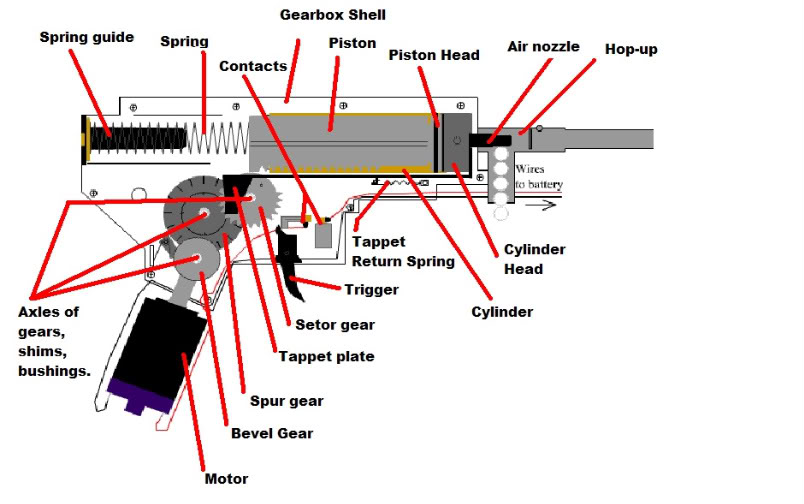
\includegraphics[width=1\linewidth]{mech_gearboxdiagram}
	\caption{V2 gearbox alkatrészei}
	\label{fig:mech_gearboxdiagram}
\end{figure}

A hop-up kamrán belül még található egy gumi csúszófelület, amivel a kilőtt golyó perdületét lehet állítani, ezáltal pedig a fegyver effektív távolságát növelni.

\ABRAKELL

A gearbox-on belül kellett alakítanom a működésen, hogy az előbb leírt folyamatos működést biztosítani tudjam.  Az elsütőbillentyűt, a tűzkapcsolót és minden ehhez tartozó mechanikai elemet kiszereltem, illetve áthuzaloztam. Erre azért volt szükség, mert különben csak a ravasz meghúzásával lehetett volna tüzelni, ami bonyolít a rendszer megvalósításán. A gearbox belső kialakítása a \ref{fig:gearboxbele}. ábrán látható.

\begin{figure}[h!]
	\centering
	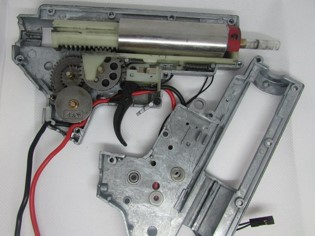
\includegraphics[width=0.6\linewidth]{gearboxbele}
	\caption{A gearbox belseje}
	\label{fig:gearboxbele}
\end{figure}

A fegyver gearbox-ot körülvevő alkatrészeiről le tudtam venni méreteket, ez alapján alakítottam ki később a 3D nyomtatott alkatrészeket. Így végeredményben egy magába zárt alkatrészem lett, amin habár mechanikus nem lehet állítani a tüzelés módját, de csupán két vezetékkel csatlakozik az elektronikához. \\

A gearbox áramfogyasztását illetően találtam méréseket az internet, ahol kifejezetten az én modellemet tesztelték. Az Itteni mérések alapján arra következtettem, hogy 15 A-re méretezni az áramkört megfelelő lehet. \cite{aisroftteszt}

\subsubsection*{Motorok}

A projekthez kettő \textbf{NEMA-17} léptetőmotort használok\cite{nema17}. Ezek a léptetőmotorok egy széles körben alkalmazott típusa, amelyet főként precíziós mozgatási feladatokhoz használnak, például CNC gépekben, 3D nyomtatókban, robotikai alkalmazásokban és automatizálási rendszerekben. A NEMA-17 esetében a szám a motor elülső oldalának névleges méretét jelenti, amely 1.7 hüvelyk, azaz körülbelül 42,3 mm. A motorok a használt vezérlővel a \ref{fig:mech_stepper}. ábrán láthatóak.\\

\begin{figure}[h!]
	\centering
	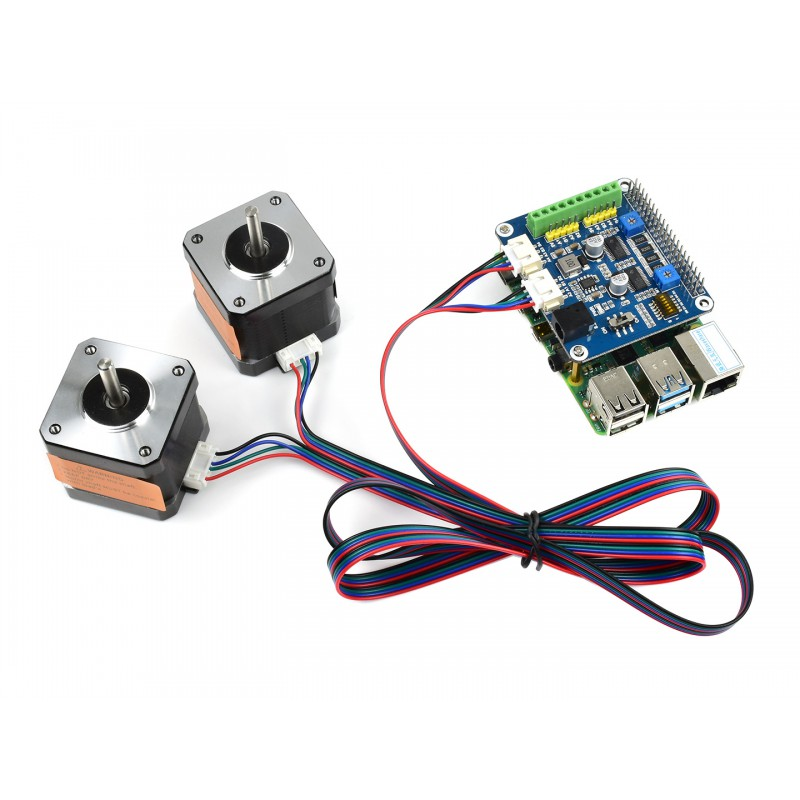
\includegraphics[width=0.8\linewidth]{mech_stepper}
	\caption{NEMA-17 léptetőmotorok a használt konfigurációban}
	\label{fig:mech_stepper}
\end{figure}

A léptetőmotorok általánosan használt típusai közé tartoznak a szervomotorok és az aszinkron motorok. A léptetőmotorok azonban a mozgásukat apró, egyenlő lépésekre osztják, így lehetővé téve a precíz pozícionálást és sebességszabályozást. A NEMA-17 léptetőmotor tipikusan kétfázisú bipoláris motor, amely négy vezetékes tekercseléssel rendelkezik. Minden lépés során a motor egy adott szöggel fordul el, ami az adott motor típusától és felépítésétől függően tipikusan 1.8 fok, így teljes fordulat esetén 200 lépésre van szükség.\\

Az én esetemben használt léptetőmotorok lépésszöge 1.8 fok, bár ezt a motorvezérlőn lehet tovább osztani. A tartónyomatéka 0.4 Nm. Ezek a paraméterek 10-es áttételű fogaskerék-kapcsolattal megfelelőnek kell lenniük egy ilyen kis teljesítményű alkalmazásnál.

\pagebreak

\subsection{3D tervezés, modellezés}
A 3D tervezést Top-Down módszerrel végeztem, ez azt jelenti, hogy először az összeállítás szintjéről kezdem a tervezést, és egy úgynevezett skeleton modellbe veszem fel az egyes alkatrészek méreteit. Ezáltal tudom garantálni az egymáshoz való illeszkedést, valamint a változtatások könnyű implementálását.\\

\subsubsection*{Skeleton modell}
A modellezést a skeleton modellek megalkotásával kezdtem. A fő összeállításon belül két skeleton modellt hoztam létre, mivel maga a modell két alösszeállítása jól elkülöníthető egymástól.

\begin{figure}[h!]
	\centering
	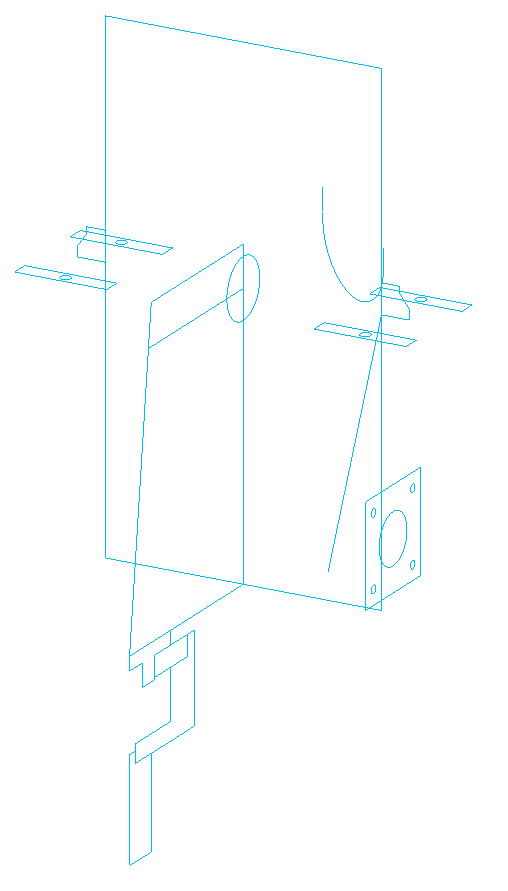
\includegraphics[width=0.5\linewidth]{mech_skeleton1}
	\caption{DT-9999 skeleton modell}
	\label{fig:mech_skeleton1}
\end{figure}

Az egyik (\ref{fig:mech_skeleton1}.ábra) alkatrészei rendszerint a függőleges tengely körül szimmetrikusak, a másiké (\ref{fig:mech_skeleton2}.ábra) pedig a fegyver csöve körül.

\begin{figure}[h!]
	\centering
	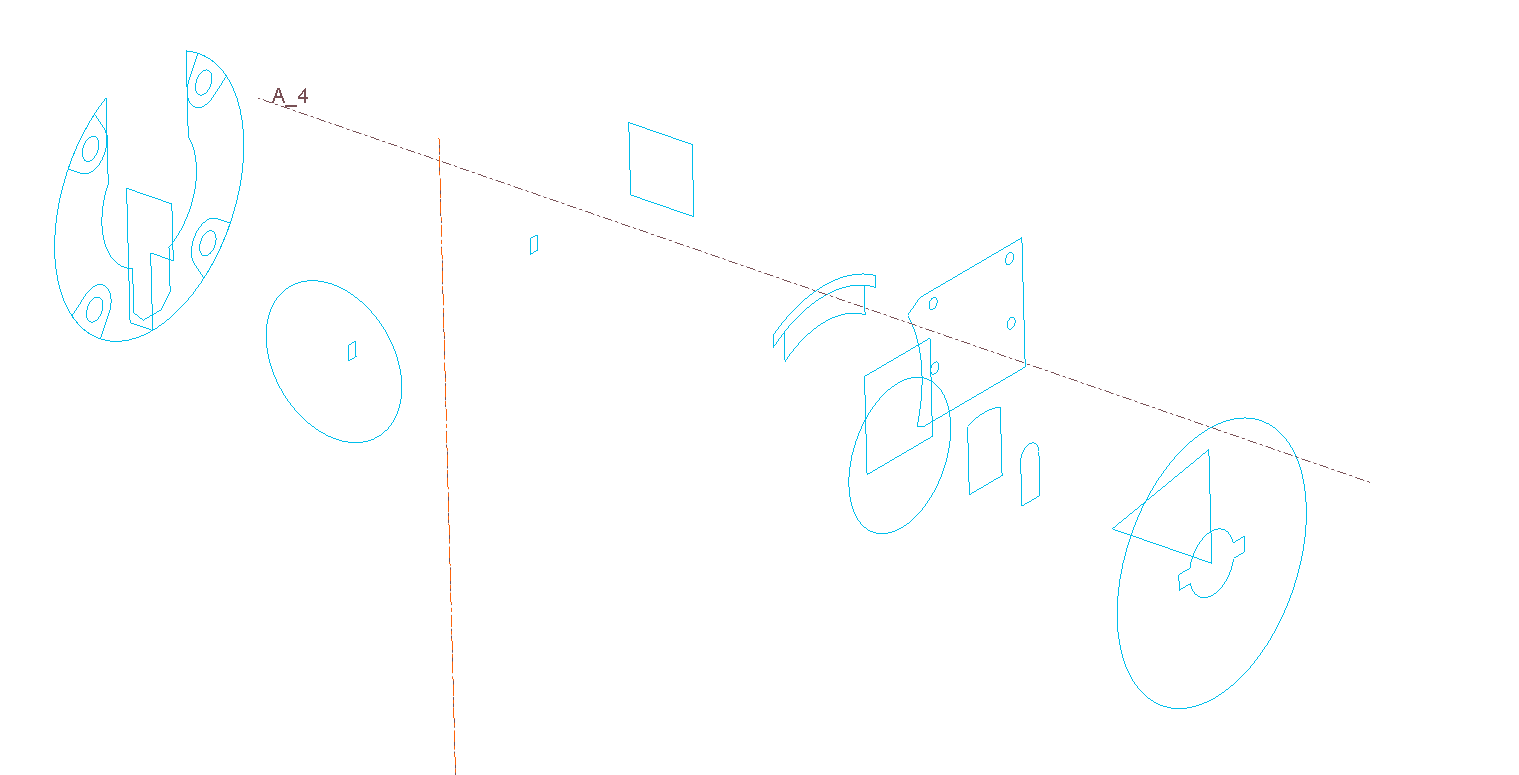
\includegraphics[width=1\linewidth]{mech_skeleton2}
	\caption{DT-4999 skeleton modell}
	\label{fig:mech_skeleton2}
\end{figure}

Az ábrákon láthatóak a vázlatok és tengelyek, amelyek alapján kialakítottam az egyes alkatrészeket. Sok méretet először csak hozzávetőlegesen vettem fel, pl. a torony magasságát. A Top-Down módszer előnye, hogy később ezeket könnyedén módosíthatom, és az alkatrészek frissítés után ugyanúgy fognak egymáshoz illeszkedni.

\pagebreak

\subsubsection{Torony}

Elsőként a \textbf{gearbox tartó elemet} kezdtem el tervezni, mert maga a gearbox volt a tervezés elején az egyetlen elem, amiből tudtam következtetni a szükséges méretekre. Erről kép a \ref{fig:mech_dt4000}. ábrán látható. 

\begin{figure}[h!]
	\centering
	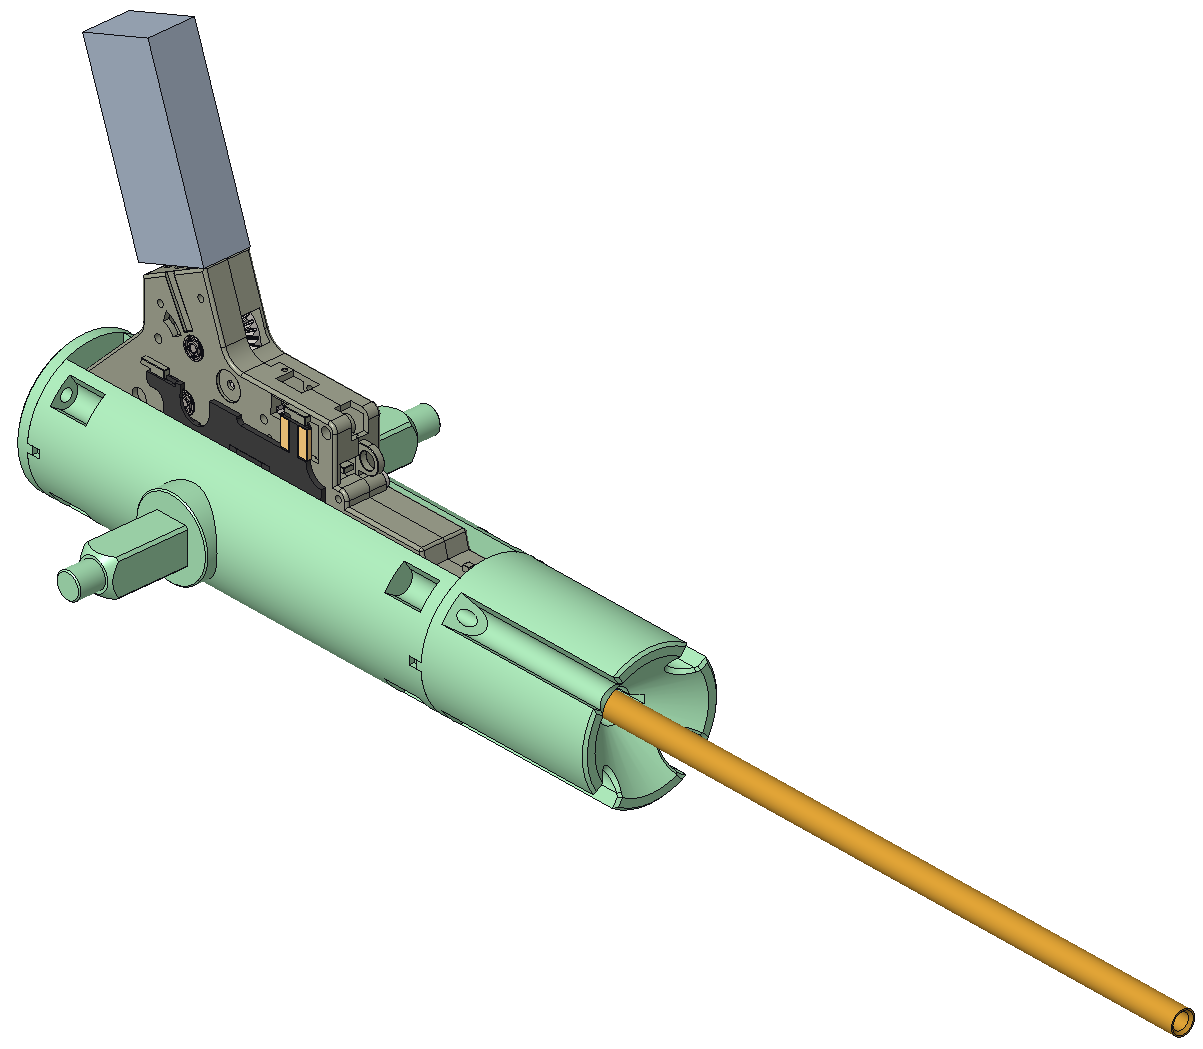
\includegraphics[width=0.8\linewidth]{mech_dt4000}
	\caption{Gearbox tartó ház}
	\label{fig:mech_dt4000}
\end{figure}

A gearbox ház 3 alkatrészből áll, egy központi elemből, valamint két fedélből a végein. A kialakítást a teljes airsoft fegyver alapján terveztem, hogy ugyanúgy álljon a gearbox mint az eredeti felhasználása során. A kritikusabb rész ebben az elemben a hop-up kamra körüli kialakítás volt, itt elég komplex volt a geometria, de a 3D nyomtatás lehetővé tette a megvalósítást. Ezt a \ref{fig:mech_dt4200}. ábrán lehet látni.


\begin{figure}[h!]
	\centering
	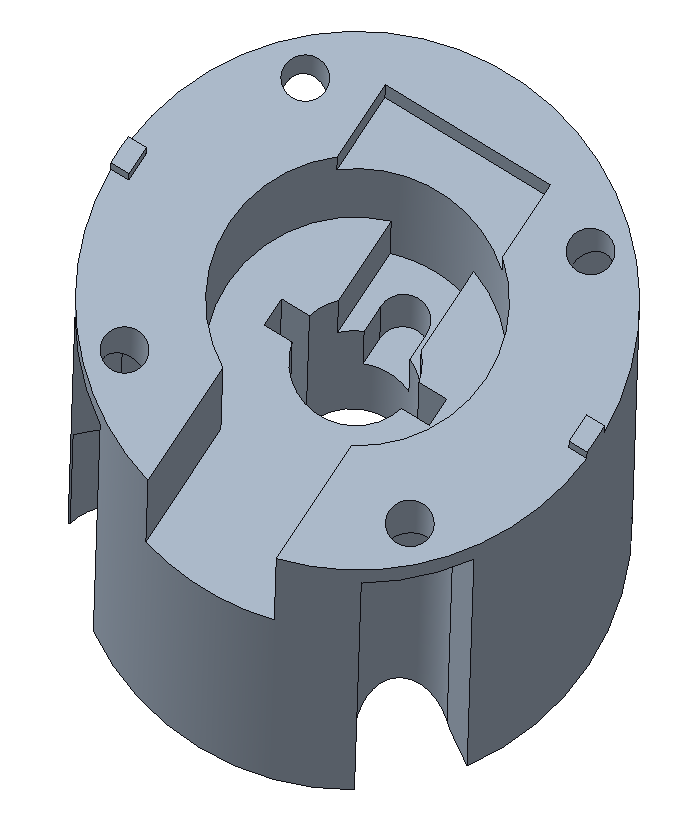
\includegraphics[width=0.4\linewidth]{mech_dt4200}
	\caption{Hop-Up kamra körüli elem}
	\label{fig:mech_dt4200}
\end{figure}


A következő alösszeállítás a \textbf{tár} volt, amely a gearbox ház bal oldali tengelyére csatlakozik. Ennek kialakítása a \ref{fig:mech_tar}. ábrán látható. A 6 mm-es golyók a zöld kupak nyílásán keresztül tölthetőek a lila tárba. Alul és felül 1-1 gumigyűrű feszíti előre a zöld dugattyút, ami a tár kúpos végén keresztül nyomja ki a golyókat. Így mechanikailag, plusz elektronika nélkül biztosítható a fegyver lövedékkel való ellátása, és szemmel is látható a tár töltöttségi szintje.

\begin{figure}[h!]
	\centering
	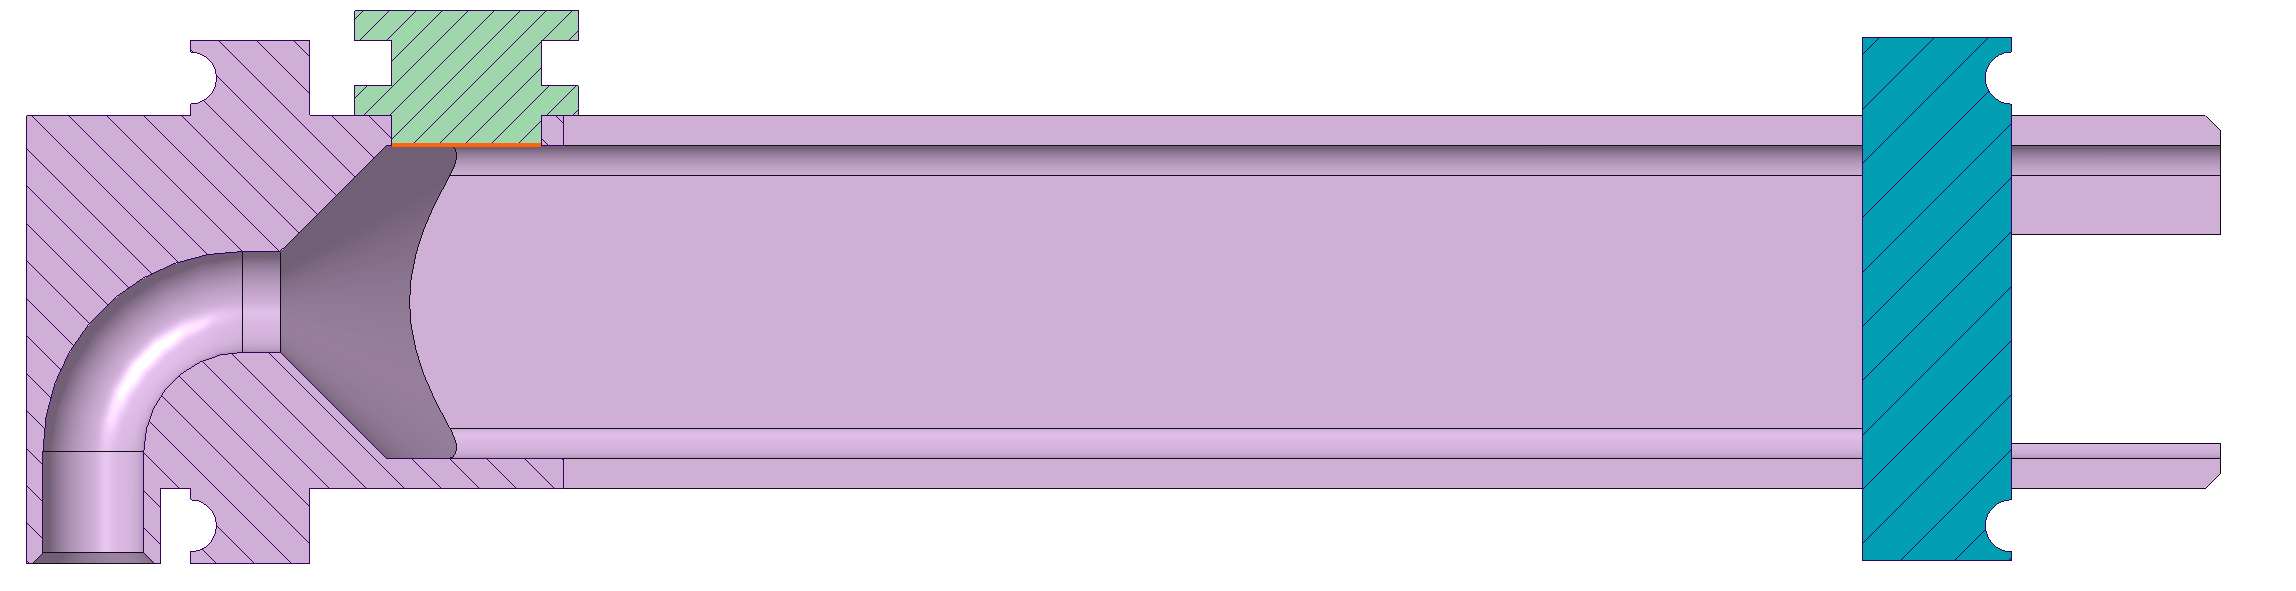
\includegraphics[width=1\linewidth]{mech_tar}
	\caption{Tár}
	\label{fig:mech_tar}
\end{figure}

Ez a kialakítás végül nem volt sikeres, ugyanis a golyók nagyon könnyedén elakadtak, gyakorlatilag egyszer sem sikerült lőni vele. Újragondolás után egy hasonló megoldást használtam, ám a golyók egyesével sorakoznak a tárban.

Végül a toronyra kerültek az elektronikai alkatrészek is, ezek a \ref{fig:mech_dt4000kamera}. ábrán láthatóak. A lila elem a lézer modul, a piros pedig a kamera konzol. Mind a kettő ragasztással kerül rögzítésre. Fontosnak tartottam, hogy ezek az elemek közvetlenül ahhoz az elemhez legyenek rögzítve, ami a fegyver csövét is pozicionálja, azonban a kamera esetén a 3D nyomtathatóság miatt egy konzolt szükségesnek éreztem.

\begin{figure}[h!]
	\centering
	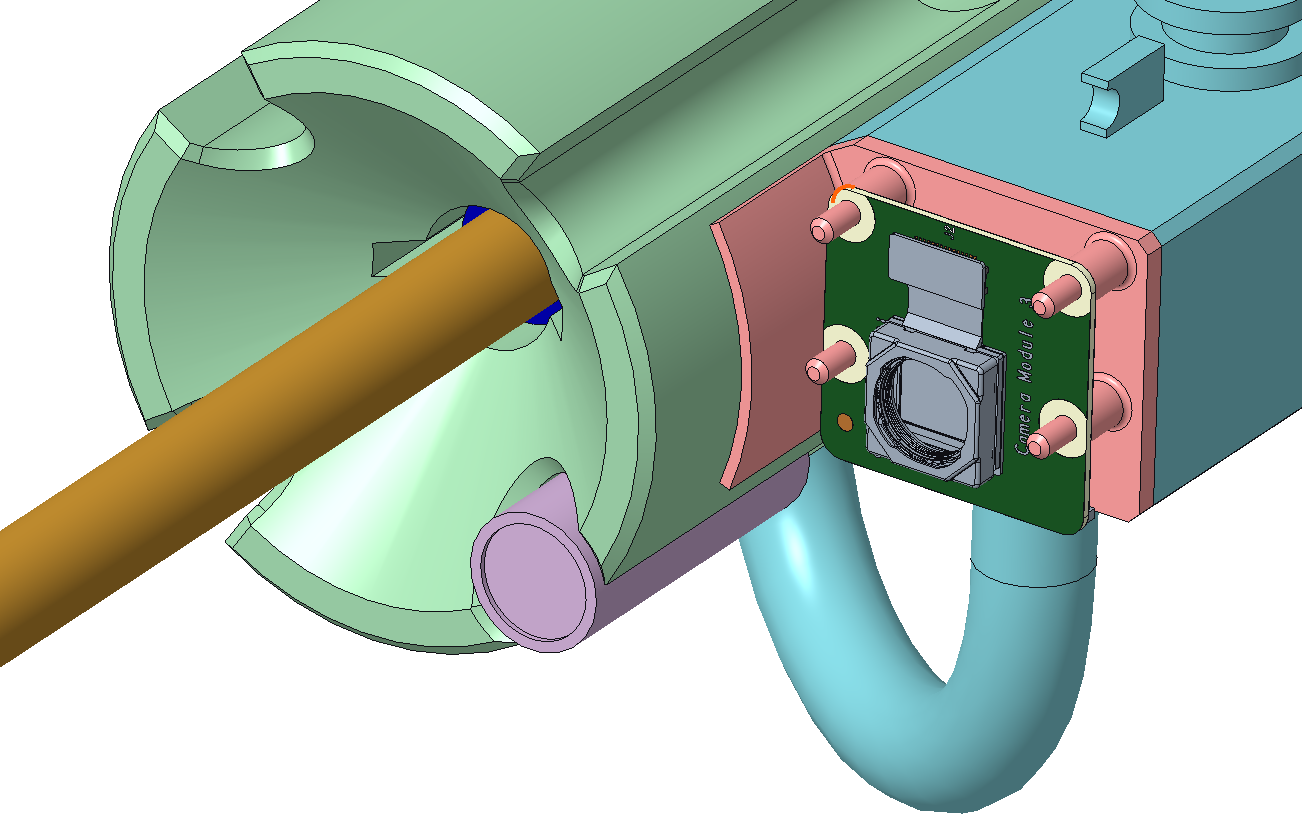
\includegraphics[width=1\linewidth]{mech_dt4000kamera}
	\caption{Kamera és lézer modul beépítés}
	\label{fig:mech_dt4000kamera}
\end{figure}

\subsubsection{Keret}
Az úgynevezett \textbf{keret} volt a konstrukció legösszetettebb eleme, és egyben a legnagyobb térfogatú is. Fő funkciója a torony stabil tartása a csapágyakkal együtt. Ezentúl erre az elemre van rögzítve a vezérlőelektronika nagy része, a végálláskapcsolók és a vízszintes tengelyhez tartozó motor is. Ez az elem az alatta lévő alkatrészhez ragasztással lett rögzítve, hogy a szerelést egyszerűsítsem. A csapágyak támasztása X elrendezésű, és az osztott "csapágyház" miatt könnyen szerelhetőek. A csapágy elrendezése  a

\begin{figure}[h!]
	\centering
	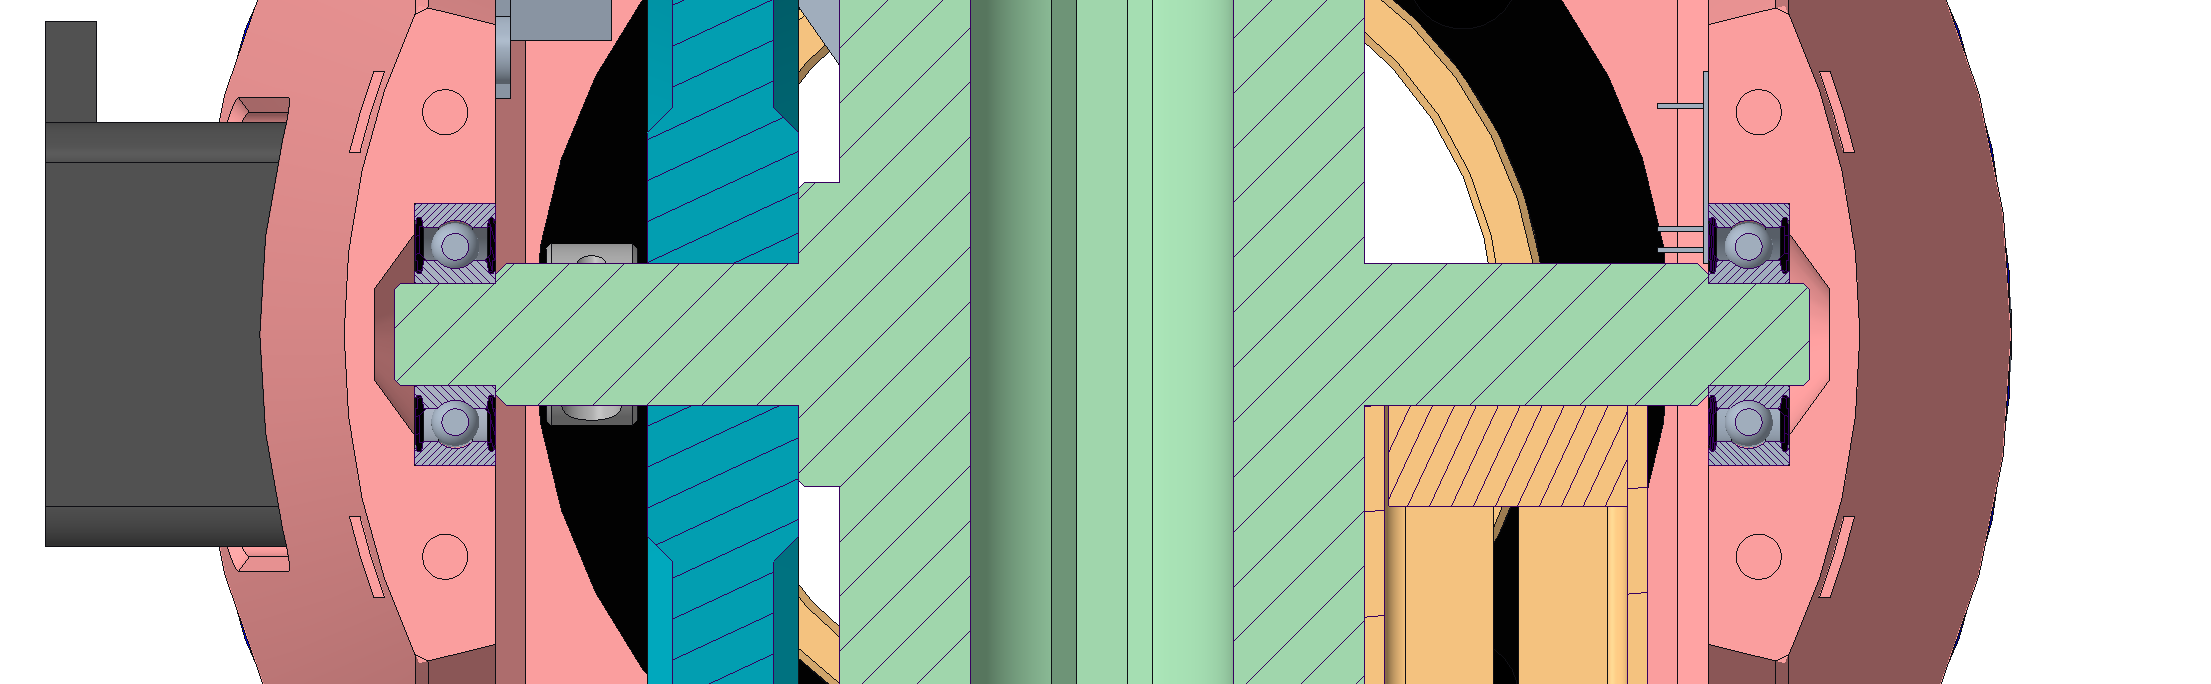
\includegraphics[width=1\linewidth]{mech_felsotengely}
	\caption{Vízszintes tengely csapágyainak elrendezése}
	\label{fig:mech_felsotengely}
\end{figure}


Kétséges rész volt a \textbf{motor} rögzítése, ugyanis nagy szükség van a pontos illeszkedésre. A nyomtatás irányára azonban a motor központosítására szánt furat pont merőleges, de szerencsére a nyomtató így is elég nagy pontosságot tudott elérni.

\begin{figure}[h!]
	\centering
	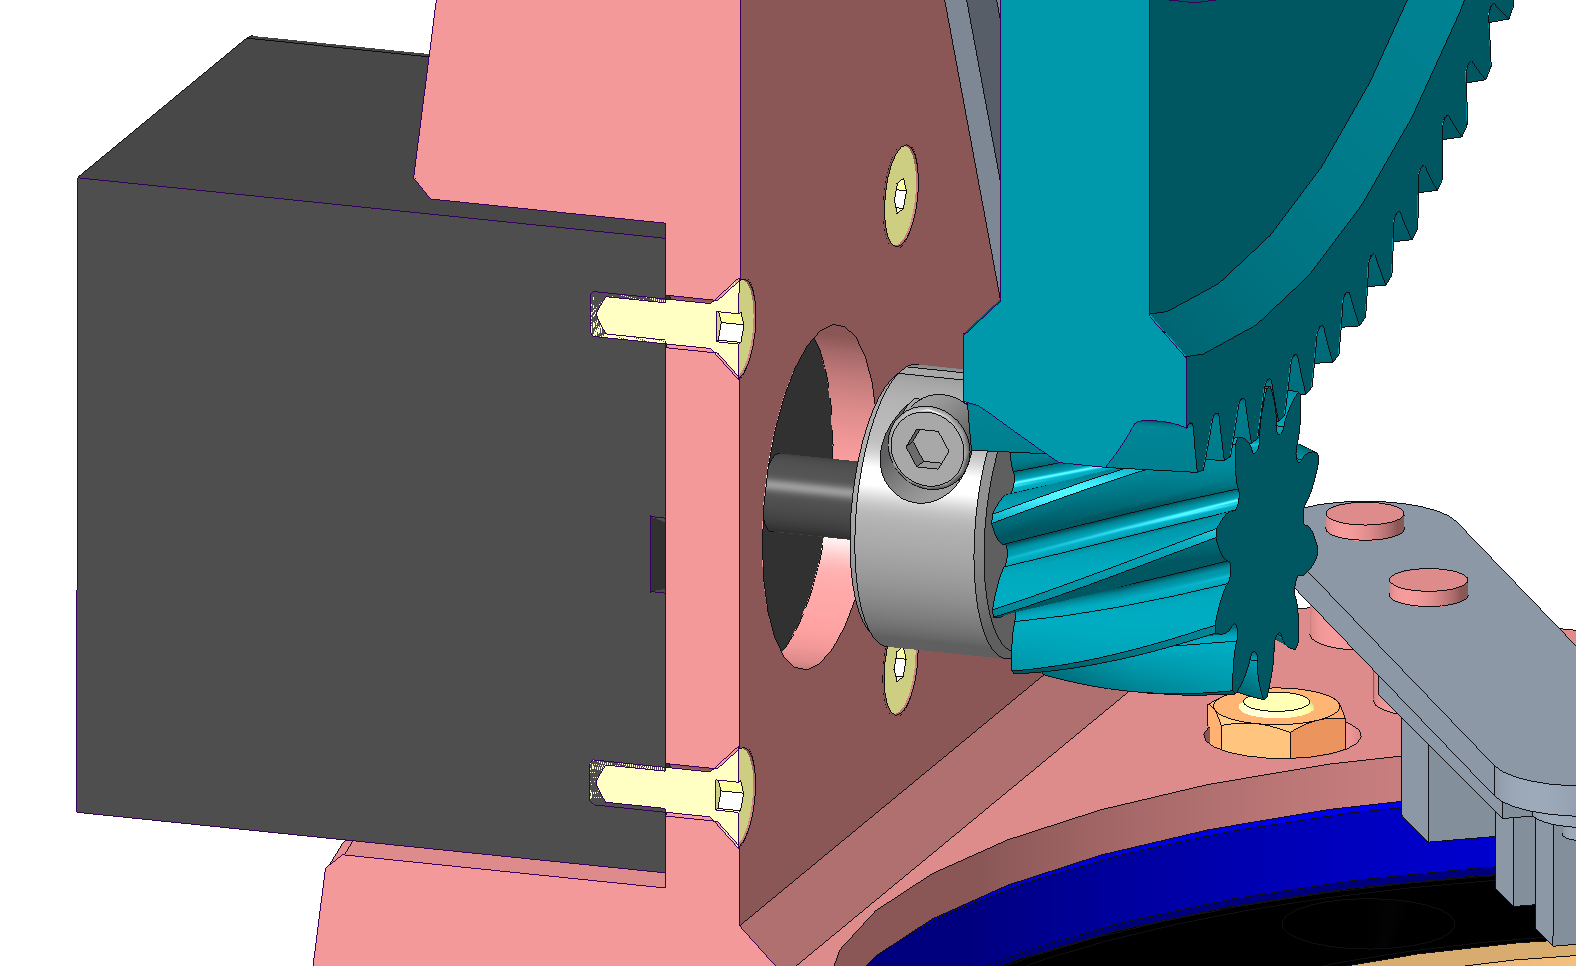
\includegraphics[width=1 \linewidth]{mech_motorbeepites}
	\caption{Vízszintes tengely motor beépítése}
	\label{fig:mech_motorbeepites}
\end{figure}

A kereten kaptak helyet a végálláskapcsolók is, amivel a rendszer indításkor kalibrálható. A egyik a vízszintes tengely nagy fogaskerekét, a másik pedig a függőleges tengely központi eleméhez viszonyít.


\begin{figure}
	\centering
	\begin{minipage}{.5\textwidth}
		\centering
		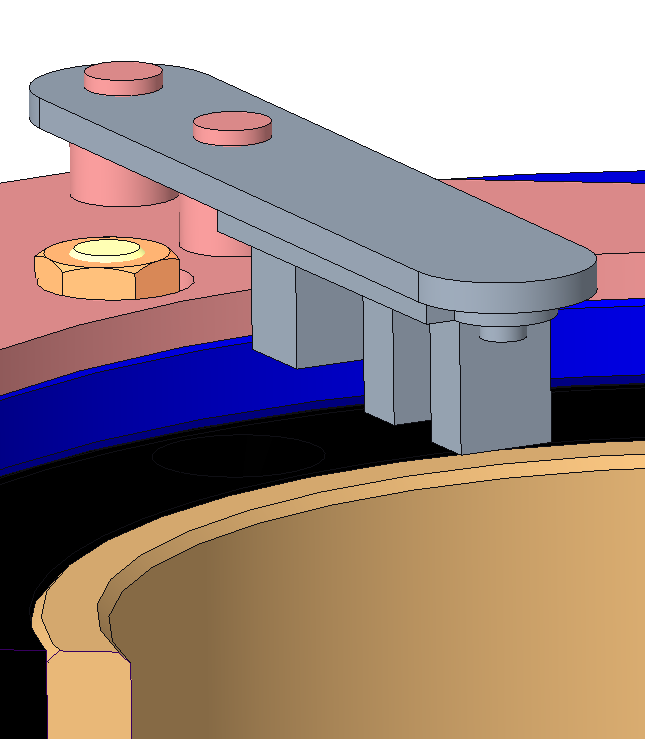
\includegraphics[width=.7\linewidth]{mech_vegallas1}
		\caption{Pan végálláskapcsoló}
		\label{fig:mech_vegallas1}
	\end{minipage}%
	\begin{minipage}{.5\textwidth}
		\centering
		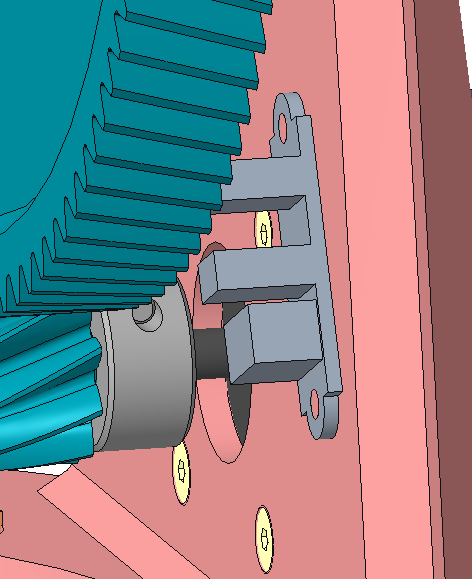
\includegraphics[width=.7\linewidth]{mech_vegallas2}
		\caption{Tilt végálláskapcsoló}
		\label{fig:mech_vegallas2}
	\end{minipage}
\end{figure}

\subsubsection{Függőleges tengely elemei}

Utolsó lépésként megterveztem a függőleges tengely mozgatásáért felelős elemeket. ezek kialakítása a \ref{fig:mech_alsoreszek}. ábrán látható. A narancssárga alakrész a központi elem, amelynek feladata a csapágy támasztása és a motor rögzítése. A motor vezetékei, valamint az elektronikából kilógó többi kábel ennek a közepén fut keresztül. A csapágy egyik fele ehhez az elemhez van rögzítve, a másik pedig  az ábrán kékkel ábrázolt alkatrészhez. Erre a kék elemere került rögzítésre a belsőfogazású fogaskerék is. \\ 

A sárga alkatrész a talapzat része. Ez a legnagyobb kiterjedésű elem az egész modellben. Hogy elkerüljem a támaszanyag használatát, a csavarok fejeinek felfekvő felületeti egy külön alkatrész ragasztásával oldottam meg. Ez a talp 45 fokos belső felületére illeszkedik, és ragasztással kerül rögzítésre. A 4 oldalán kialakításra kerültek csatlakozó felületek, ahol különböző lábak helyezhetők az eszközre.

\begin{figure}[h!]
	\centering
	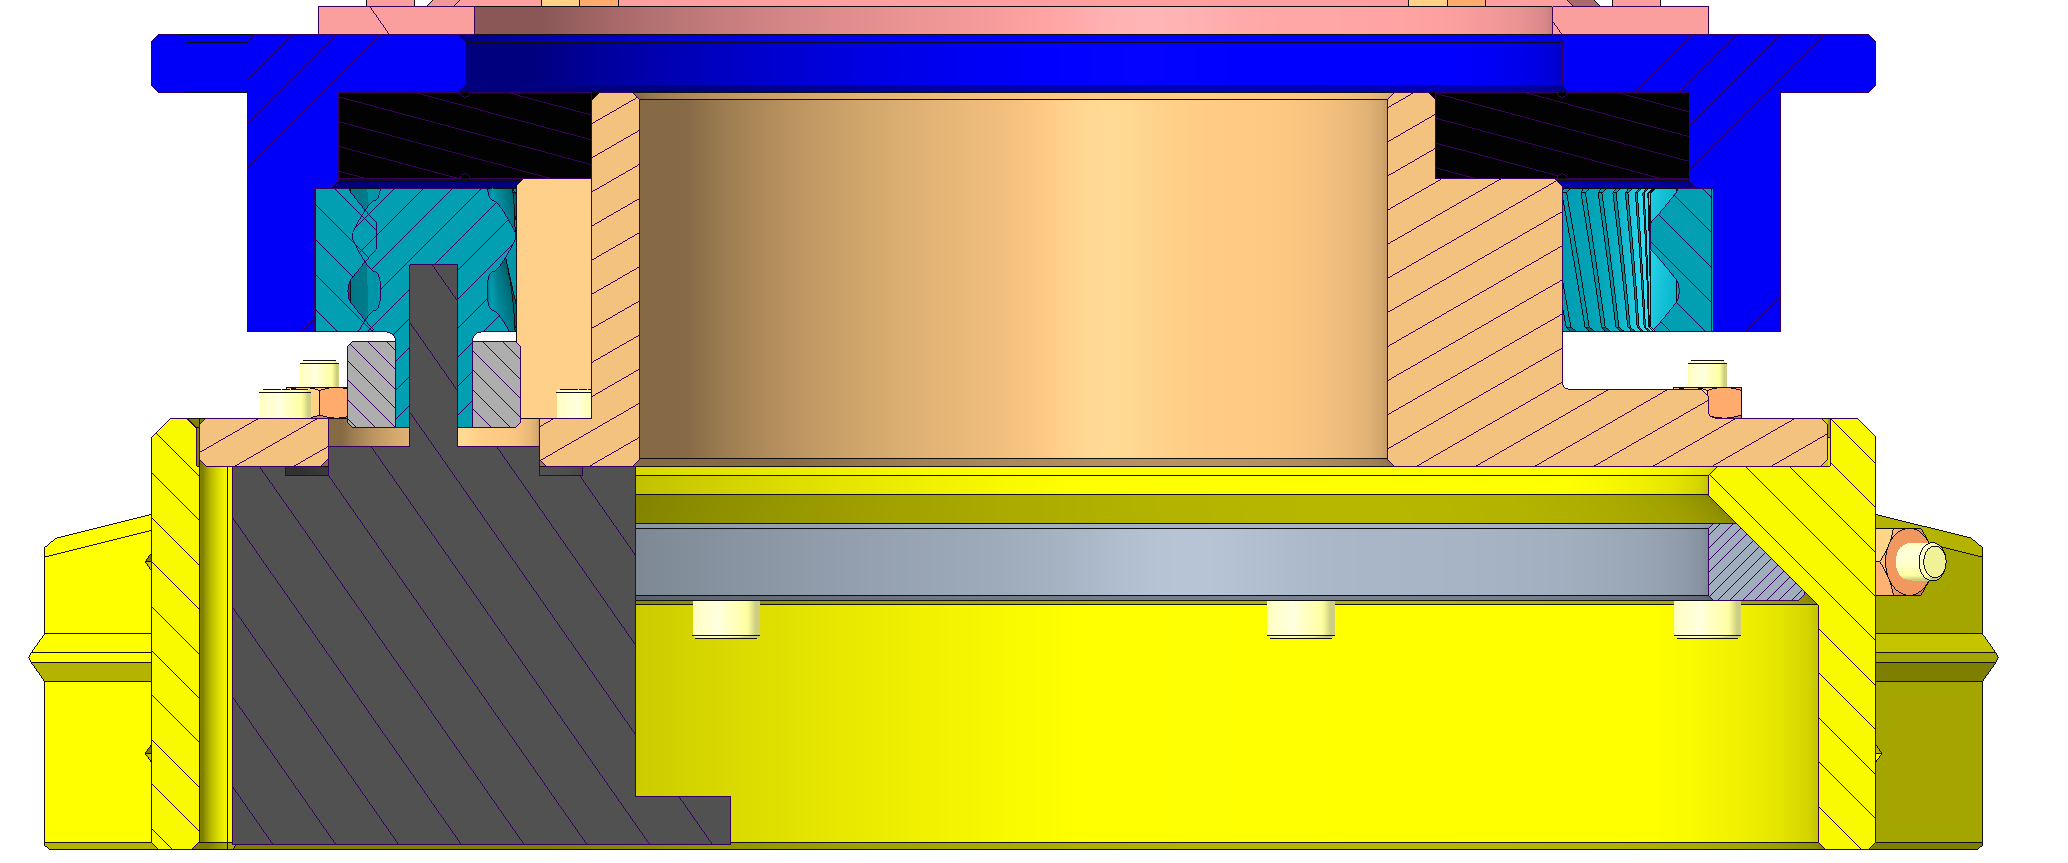
\includegraphics[width=1\linewidth]{mech_alsoreszek}
	\caption{Függőleges tengely elrendezése}
	\label{fig:mech_alsoreszek}
\end{figure}

\subsubsection{Fogaskerekek}
A prototípusban két fogaskerék kapcsolat kapott helyet. A függőleges tengely nagy fogaskereke belső fogazású, ezáltal el tudtam rejteni a motort a váz belsejében és kompaktabb lett a kialakítás, valamint valamivel stabilabb is. A kapcsolat áttétele 10, és ferde fogazású, ezáltal a futás csendesebb és egyenletesebb lett. A kapcsolat illusztrációja a \ref{fig:mech_fogpar1}. ábrán látható.

\begin{figure}[h!]
	\centering
	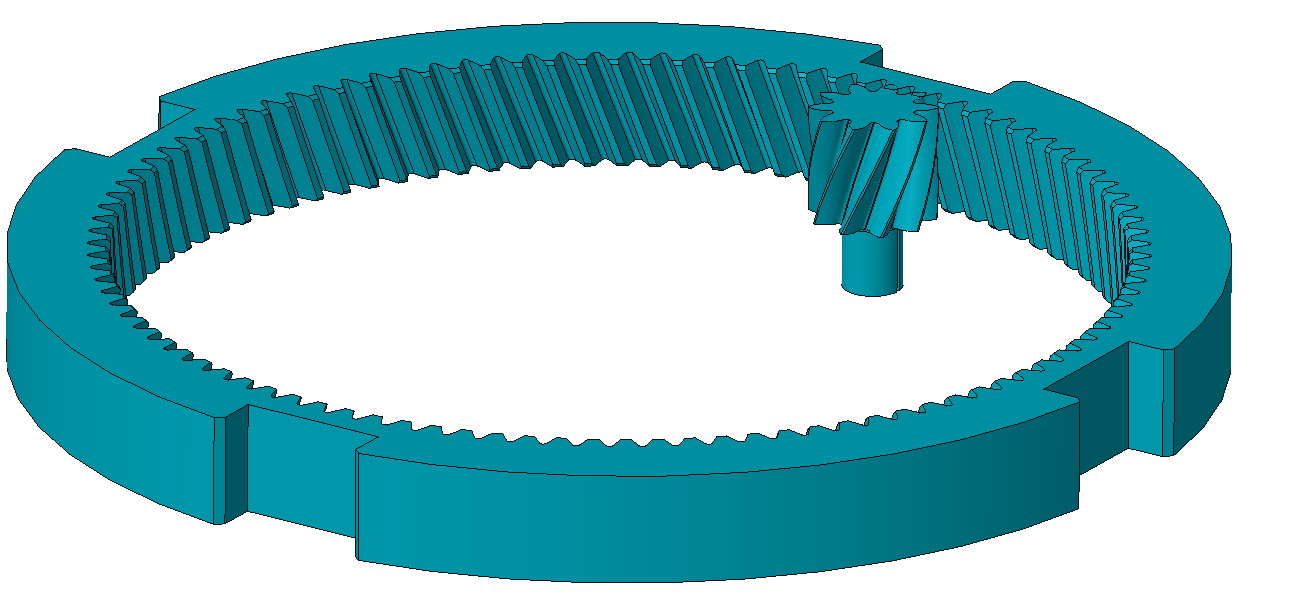
\includegraphics[width=1\linewidth]{mech_fogpar1}
	\caption{Függőleges tengely fogaskerekek}
	\label{fig:mech_fogpar1}
\end{figure}

A vízszintes tengely nagy fogaskereke a gearbox ház tengelyére lett erősítve, és csak részlegesen lett kinyomtatva. Ennek egyszerű oka, hogy más geometria is blokkolja a mozgást ezekben a tartományokban, illetve a Pan-Tilt kinematika mozgása redundáns lenne, ha teljesen körbe tudna forogni. A kapcsolat a \ref{fig:mech_fogpar1}. ábrán látható.

\begin{figure}[h!]
	\centering
	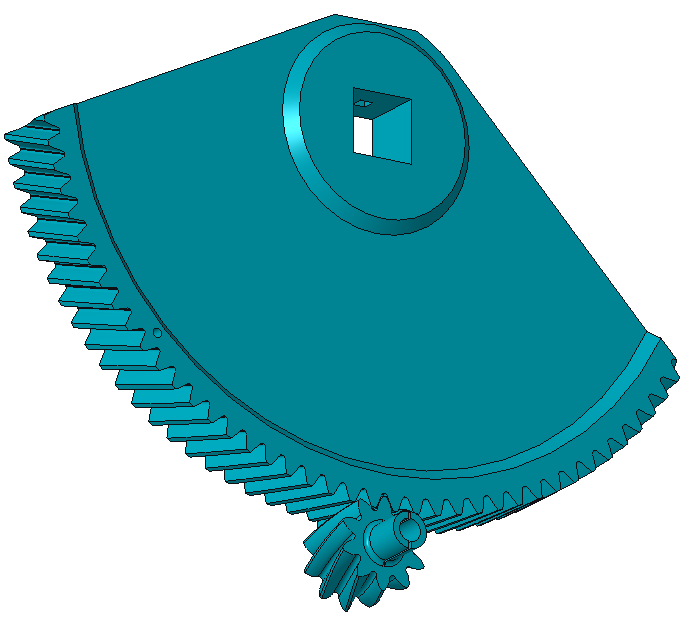
\includegraphics[width=0.7\linewidth]{mech_fogpar2}
	\caption{Vízszintes tengely fogaskerekek}
	\label{fig:mech_fogpar2}
\end{figure}

Mind a két fogaskerékpár kisebb közvetlenül a motor tengelyére lett rögzítve, egy acél rögzítőgyűrűvel. Ennek kialakítása a \ref{fig:mech_alsoreszek}. ábra bal oldalán látható.

\subsection{Gyártás és összeszerelés}
a

\pagebreak
\section{Hardvertervezés}

\subsection{Áramköri tervezés}
A prototípus áramkörét próbáltam minél egyszerűbben megvalósítani. Alapvetően két részből áll, a Raspberry PI központú vezérlőáramkörből, ami felelős a szenzorokért és a Raspberry PI-ért, illetve egy nagyobb teljesítményű áramkör egy külön tápról, ami a gearbox működtetéséért felelős.


\begin{figure}[h!]
	\centering
	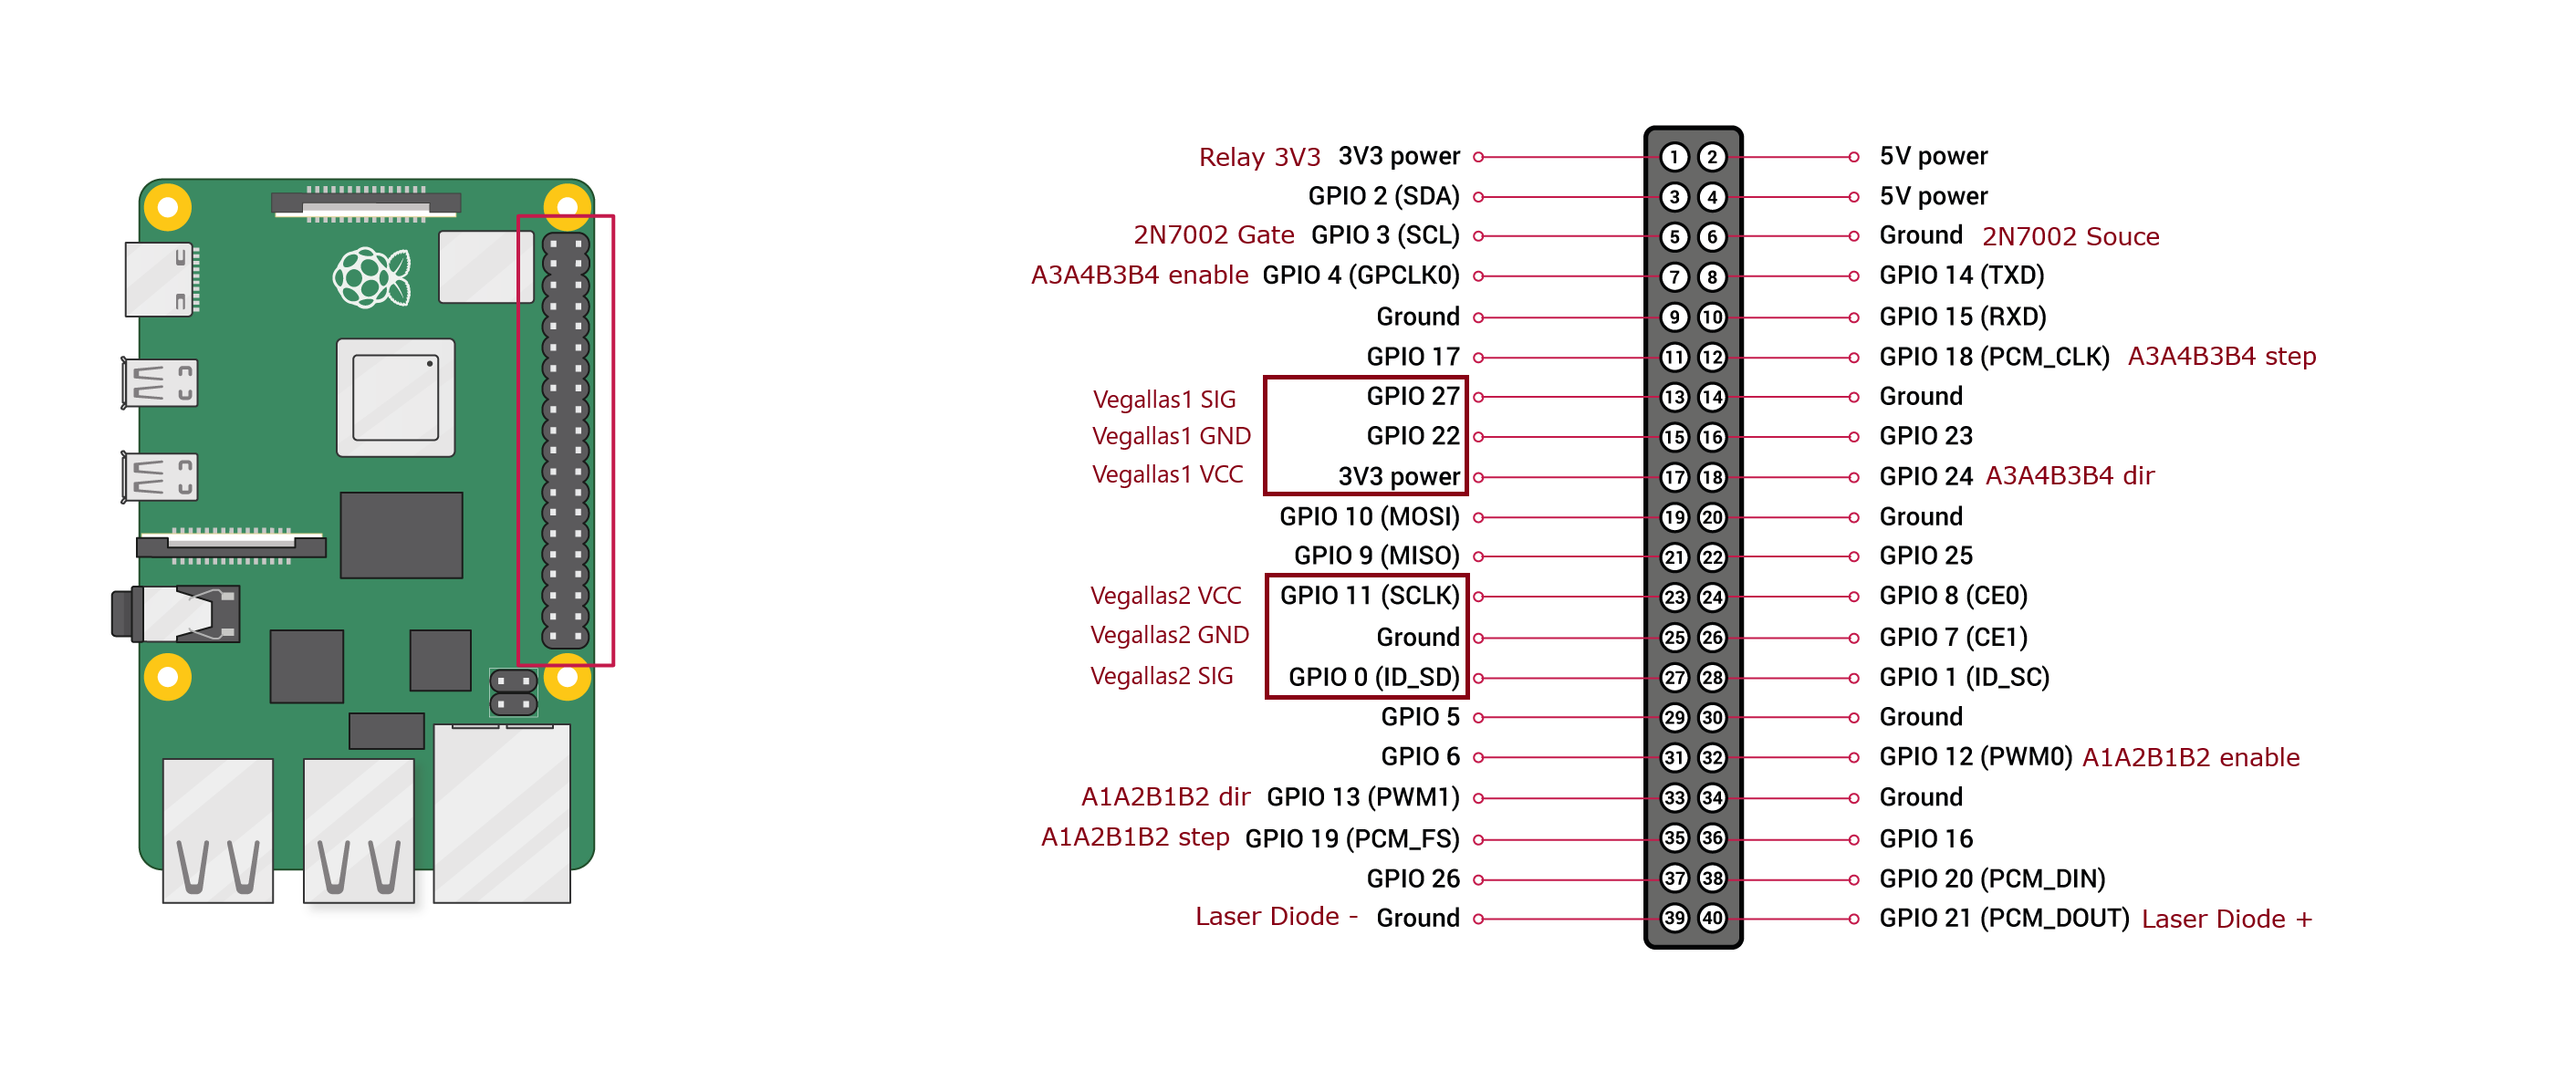
\includegraphics[width=1\linewidth]{elek_pinout}
	\caption{A Raspberry PI lábkiosztása}
	\label{fig:elek_pinout}
\end{figure}

<<<<<<< Updated upstream
A prototípus áramköre a \ref{valami} ábrán látható. A kereskedelemben kapható stepper motor HAT nagyban leegyszerűsítette a tervezés folyamatát, a segítségével nem kellett megterveznem a motorvezérlők áramkörét, illetve ezeknek az áramellátását. A \ref{fig:elek_pinout}.ábrán látható, motorokra vonatkozó jelölések szerinti GPIO lábakat a stepper motor HAT ugyan lefoglalja, de a kártya tetején lévő tüskesor ugyanúgy elérhető marad, így oda kell figyelnem, hogy ezeket a lábakat ne használjam. \\

Ahogy az ábrán látható, a végálláskapcsolók is a GPIO tüskesorra lett csatlakoztatva. Az egyiknél a földet helyettesíti GPIO22 láb, a másiknál a 3.3 V-t helyettesíti a GPIO11. Azért kellett ezt a megoldást alkalmaznom, mert a kábel csatlakozója egyben van, nem különálló jumper tüskék.\\

A lézer közvetlenül a GPIO21 lábról működik. Eleinte aggódtam, hogy nem tud elegendő áramot szolgáltatni a dióda működtetéséhez, de szerencsére mégis. Ellenkező esetben ki kellett volna egészítenem az áramkört egy tranzisztorral. \\

A relé kapcsolásához viszont nem volt elegendő a GPIO láb által szolgáltatott áram, így azt egy tranzisztorral vezérlem. Amennyiben logikai magas jelet kap, a relé zárja a gearbox áramkörét, és az elkezd lőni.
=======
Az eszköz sémarajza az alábbi ábrán látható:

\begin{figure}[h!]
	\centering
	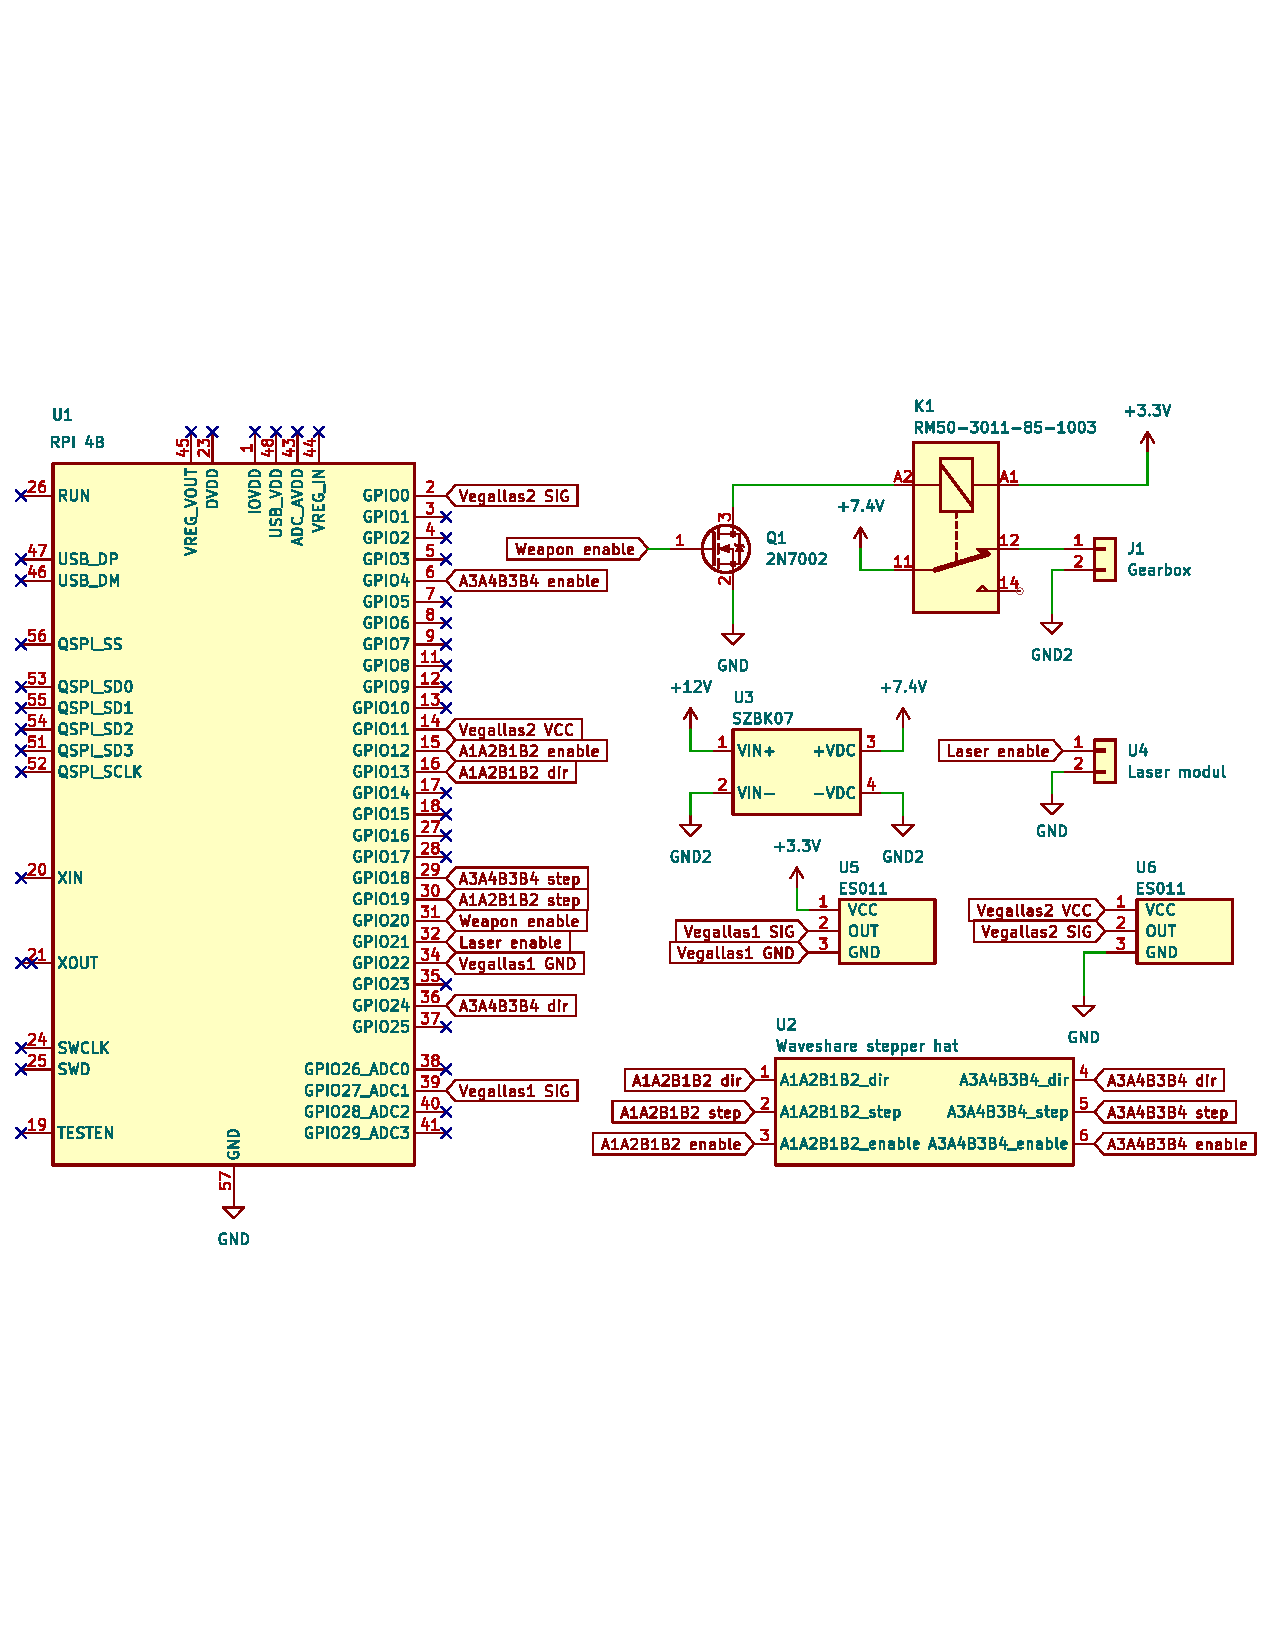
\includegraphics[width=1\linewidth]{schematic}
	\caption{A prototípus sémarajza}
	\label{fig:schematic}
\end{figure}
>>>>>>> Stashed changes

\subsection{Elektronikai alkatrészek}
\subsubsection*{Mikrovezérlő}
A mikrokontroller kiválasztásánál több opciót vizsgáltam, többek között az {Arduino}, az \textsl{STM-32} és a \textsl{Raspberry PI} modelleket. A követelmények a következőek voltak:

\begin{list}{-}{}
	\item Legyen könnyen beszerezhető, mind anyagilag, mind elérhetőség szerint
	\item Megfelelő teljesítmény gépi látás algoritmusokhoz
	\item Elegendő számú GPIO kimenet
	\item Python programozási nyelve támogatása
	\item Ethernet port
\end{list}

Azonban ahogy összehasonlítottam a különböző opciókat, körvonalazódott, hogy a \textsl{Raspberry PI} lesz a megfelelő megoldás. az eszköz a \ref{fig:elek_raspberry4b}. ábrán látható Először is egy gyakorlati szempont szerint, mégpedig hogy egy Raspberry PI 4B modell eredetileg is volt a tulajdonomban 4GB rammal. A gyártó hivatalos fórumán több felhasználó szerint ez már elegendő összetettebb gépi látás algoritmusok futtatására is. \cite{4gbforum} \\

\begin{figure}[h!]
	\centering
	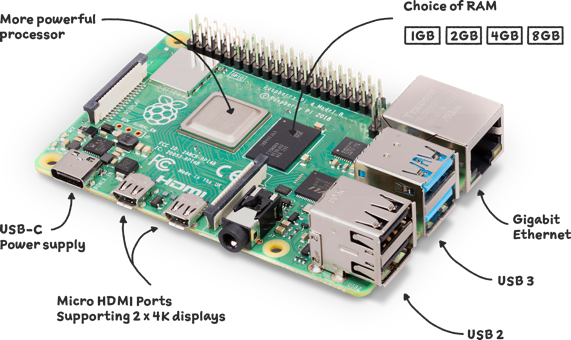
\includegraphics[width=1\linewidth]{elek_raspberry4b}
	\caption{Raspberry 4 model B}
	\label{fig:elek_raspberry4b}
\end{figure}

A kamera illesztése szintén különösen fontos a végtermék működése szempontjából, és ezen a területen magasan kiemelkedik a Raspberry a többi mikrovezérlő közül, mivel magán a gyártó a termékcsaládon belül ajánl több jó minőségű, könnyen beszerezhető kamera modult, amik illesztése már kiforrott az összes Raspberry-hez.\\

Ezentúl a \textsl{Raspberry PI} erősebb, mint a fentebb említett mikrokontrollerek. Linux rendszert futtat, és lehet rajta Python nyelven programozni, ami gépi látás, automatizálás projekteknél hatalmas előny. Számos ki-és bemenete van, ráadásul támogatja a \textsl{Bluetooth}, \textsl{Wi-Fi}, és gigabites \textsl{Ethernet} kapcsolatokat is, nem beszélve a rengeteg bővítő "kabátról", amiket lehet kapni hozzá. Ezek a termék továbbfejlesztését nagyban könnyítik, ráadásul kevesebb munkát kell a nyomtatott áramkör tervezésébe tenni. \cite{raspberry4}

\subsubsection*{Stepper Motor HAT}
A NEMA-17 léptetőmotorok vezérlésére több megoldás is létezik, elterjedtek a \textsl{A4988}, \textsl{TMC5160T} és \textsl{DRV8825} típusú vezérlők. Ezeket azonban vagy külön modulként lehet megvásárolni, vagy pedig SMD alkatrészként, ami mellé mindenképpen kell tervezni kiegészítő áramkört. \\

Azonban a \textsl{Waveshare} cég gyárt egy Raspberry Pi-kompatibilis modult, ami számomra rengeteg segítséget nyújtott. Ez egy külön áramkör, amit a Raspberry GPIO tüskesorára lehet illeszteni. Képes két \textsl{DRV8825} vezérlővel egyszerre kettő léptetőmotort vezérelni. A kártyán lévő kapcsolókkal könnyen lehet állítani külön motoronként a microsteppelést is, amennyiben szükség van rá egészen 1/32-ig. A potméterekkel motoronként tudjuk állítani a maximális felvehető áramot, maximum 2.5 A-ig. A kártyán helyet kapott egy standard 5.5 mm-es csatlakozó is, amivel 8.2 V és 28 V közötti feszültséggel lehet táplálni az áramkört. Egy belső regulator chip segítségével a Raspberry PI-t is el lehet látni árammal, így egy tápegységgel tudom működtetni a teljes áramkört. A modulon több lehetőség is van csatlakoztatni a motorokat, akár sorkapoccsal, akár a léptetőmotorok szabvány csatlakozójával. Ezentúl lehetővé teszi a Raspberry PI GPIO lábainak elérését, csupán arra kell odafigyelni, melyikeket használja. Az eszközről a \ref{fig:elek_stepperhat}. ábrán látható illusztráció. \cite{stepperhat}

\begin{figure}[h!]
	\centering
	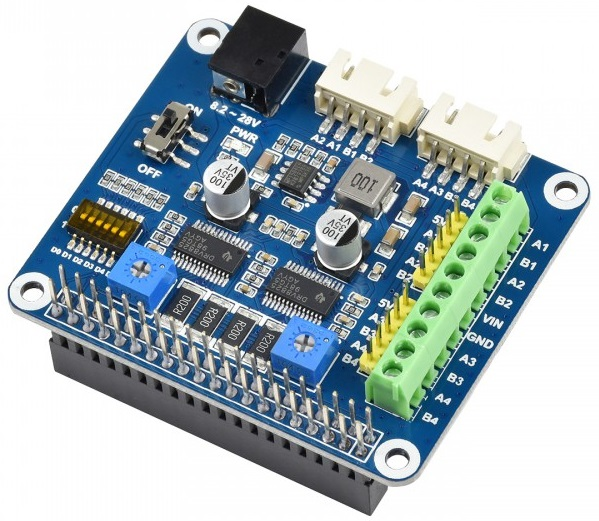
\includegraphics[width=1\linewidth]{elek_stepperhat}
	\caption{Waveshare Stepper HAT}
	\label{fig:elek_stepperhat}
\end{figure}

Az eszköz el lett látva különböző biztonsági funkciókkal, pl. túláram védelemmel, magas hőmérséklet elleni védelemmel, illetve alulfeszültség lockout-tal.\\

A gyártó szintén elérhetővé tett illesztőszoftvereket több eszközre, több motortípusra, amit a későbbiekben én is tudtam használni.

\subsubsection*{Táp}

A prototípust két tápegységről működtetem. Az egyik a Raspberry PI, a léptetőmotorok és a szenzorok áramellátásáért, ez egy standard 5.5 mm-es csatlakozóval ellátott laptop töltő. 14.5 V tápfeszültséget és maximum 5 A áramot képes biztosítani, amely bőven elegendő a vezérlőelektronika ellátására.

\ABRAKELL

A másik táp egy \textsl{HP ps-3701-1} 12 V-os redundáns szervertáp 725 W teljesítménnyel. 

\subsubsection*{Kamera}
A rendszer által használt kamera egy \textsl{Raspberry Pi Camera Module 2} volt.\cite{raspberrycam} Ez a modul 8 MP-es \textsl{Sony IMX219} szenzorral rendelkezik, amivel 3266 x 2450 felbontású állóképet tud készíteni. Képes Full HD videót felvenni 30 fps-el, HD-t 60 fps-el, vagy 640x480 felbontást 90 fps-el. A modul a \ref{fig:elek_raspberrycam}. ábrán látható.

\begin{figure}[h!]
	\centering
	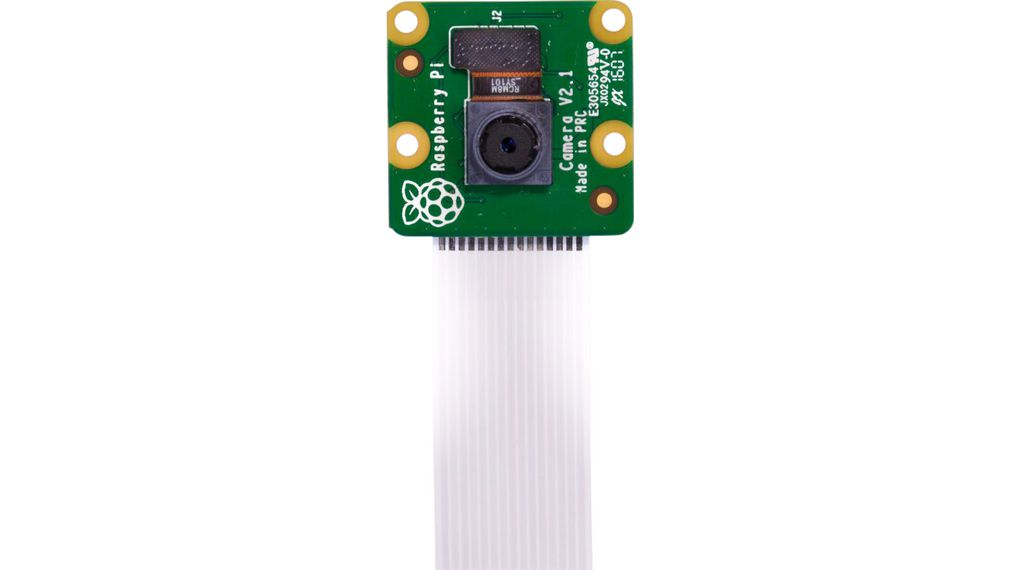
\includegraphics[width=1\linewidth]{elek_raspberrycam}
	\caption{Raspberry Pi Camera Module 2}
	\label{fig:elek_raspberrycam}
\end{figure}

A kamera befoglaló mérete szerelési furatai és CSI portja megegyezik a többi Raspberry kamerával, így a továbbfejlesztés esetén könnyedén lehet őket cserélni.

\subsubsection*{Végálláskapcsoló}
A prototípus bekapcsolásánál fontos, hogy beálljon egy kezdőpozícióba, és ahhoz képest tudjuk viszonyítani a mozgását. Ezt én a két tengelyen 1-1 végálláskapcsolóval oldottam meg. Ezek a modulok könnyen szerelhetőek a 3D nyomtatott vázra, és az alapján adnak jelet, valami van-e az optokapu között. A Raspberry GPIO lábaira könnyedén lehet őket bekötni jumper kábelek segítségével. A szenzorok a \ref{fig:elek_vegallaskapcsolo}. ábrán láthatóak.

\begin{figure}[h!]
	\centering
	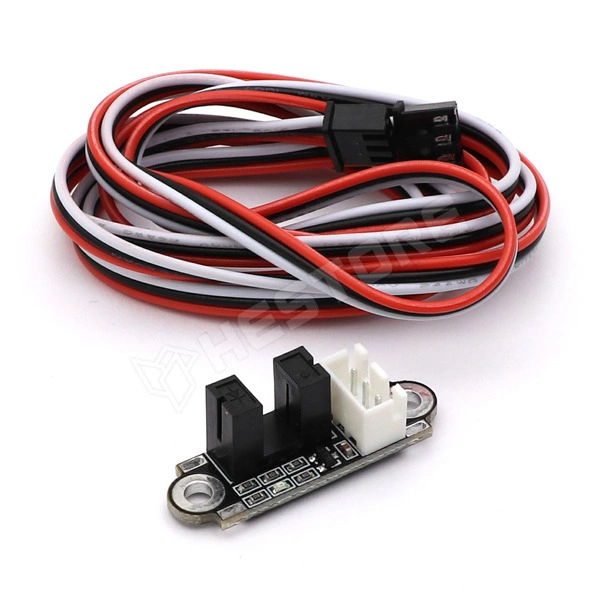
\includegraphics[width=0.5\linewidth]{elek_vegallaskapcsolo}
	\caption{Végálláskapcsoló}
	\label{fig:elek_vegallaskapcsolo}
\end{figure}

\subsection{Gyártás, forrasztás}
A projekthez egyedi nyomtatott áramkört nem kellett gyártatni, azonban egy kis forrasztást igényelt. A gearbox táp folyamatos működéséhez az alább látható módon kellet egy huzallal összeforrasztanom a padokat. Látható a 12V és GND-hez csatlakozó kábelek is, amiket szintén beforrasztottam a megfelelő helyre. Ezen a területen van lehetőség a továbbfejlesztésre, például egy 3D nyomtatott elemmel.\\

Ezentúl a kábeleket kellett forrasztanom, illetve a relé és a hozzá tartozó tranzisztor áramkörét. Ezek az alábbi képen láthatóak. Azokat a kábeleket, ahol nagyobb áram folyhat, és szerettem volna, hogy szerelhetőek legyenek, ott WAGO 221 összekötőkkel oldottam meg a csatlakozást.

\pagebreak

\section{Szoftverfejlesztés}
A prototípus szoftverét kettéválasztottam a két működési mód szerint, az egyik a manuális vezérlést valósítja meg, a másik az automatikust. A kettő között lényeges különbségek vannak a prioritásokban. A kézi vezérlésnél a legfontosabb a valós idejű megjelenítés, és a minél gyorsabb reagálás a felhasználói parancsokra. Az automata működésnél a megjelenítés kevésbé fontos, viszont a képfelismerés és ez által a célpont követése kiemelkedő fontosságú.


\subsection{Használt Python modulok, eszközök}
\subsubsection*{OpenCV könyvtár}
Az \textbf{OpenCV} (Open Source Computer Vision Library) egy nyílt forráskódú könyvtár, amelyet eredetileg az Intel fejlesztett ki, és amelyet széles körben használnak a számítógépes látás (computer vision) és képfeldolgozás területén. Az OpenCV rendkívül sokoldalú eszközkészletet biztosít a képekkel és videókkal kapcsolatos különféle feladatok megoldásához, amelyet elsősorban C++-ban fejlesztettek ki, de támogat Python, Java, és MATLAB interfészeket is. A Python interfész különösen népszerű, mivel egyszerűsíti az OpenCV használatát gépi tanulási és mesterséges intelligencia-alkalmazásokban. A fő funkciói közé tartozik a képfeldolgozás, tárgy- és arcérzékelés, mozgáskövetés, valamint a 3D-s modellezés és képanalízis.\\

Az OpenCV architektúrája moduláris felépítésű, ami lehetővé teszi a különböző funkciók rugalmas használatát. A modulok között megtalálhatóak a képfeldolgozási, objektumfelismerési, gépi tanulási és 3D modellezési könyvtárak. A Pythonban a \code{cv2} könyvtárként importálható OpenCV API biztosítja a különböző funkciók egyszerű elérését, így akár néhány sor kóddal is gyors eredmény érhető el.\\

Többféle képformátumot támogat, például JPEG, PNG és BMP, és rendelkezik valós idejű video- és képadatok betöltésére szolgáló funkciókkal is, például a \code{VideoCapture} objektummal. Ez utóbbi lehetővé teszi, hogy közvetlenül kamerákból vagy videófájlokból dolgozzunk.\\

Az \textbf{OpenCV }használata igen elterjedt az iparban és a kutatásban is, többek között autonóm járművek, biztonsági rendszerek, gyártósori ellenőrző rendszerek, orvosi képalkotás és mobilalkalmazások terén. A könyvtár rugalmassága és széleskörű támogatása lehetővé teszi, hogy számos programozási és mérnöki területen is alkalmazható legyen, ahol képfeldolgozásra és gépi látásra van szükség.

\subsubsection*{Socket modul}

Python \code{socket} modulja alacsony szintű hozzáférést biztosít a hálózati kommunikációhoz, lehetővé téve különböző típusú hálózati kapcsolatok létrehozását, beleértve az általam használt TCP-t és az UDP-t.\\

A \textbf{TCP} kapcsolat-orientált protokoll, amely biztosítja az adatok érkezési sorrendjét és helyességét. A \code{socket.SOCK\textunderscore STREAM} típust használjuk, ha TCP kapcsolatot szeretnénk létrehozni. A TCP kapcsolatok esetében a \code{connect()} függvény a kapcsolat kezdeti lépése, és a kliens-szerver kommunikáció folyamatosan fennmarad.\\

Az \textbf{UDP} kapcsolatnélküli protokoll, amely nem garantálja az adatok sorrendjét és integritását, viszont gyorsabb, mivel nincs szükség kapcsolatra. Az UDP kapcsolathoz a  \code{socket.SOCK\textunderscore DGRAM} típust használjuk, így a kliens és a szerver bármikor küldhet és fogadhat adatokat. Ideális valós idejű alkalmazásokhoz, ahol nem kritikus minden csomag megérkezése (pl. video streaming).\\

Mindkét típusnál a \code{send()}, \code{sendto()}, \code{recv()}, és \code{recvfrom()} függvények használhatók az adatok küldésére és fogadására.

\subsubsection*{Multiprocessing modul}

A \textbf{multiprocessing} modul lehetővé teszi a Python számára, hogy párhuzamosan több folyamatot indítson el, ami segít a CPU-erőforrások jobb kihasználásában. A modul az operációs rendszer által kezelt különálló folyamatokat hoz létre, így azok külön memóriaterülettel rendelkeznek, és jobban teljesítenek többmagos processzorokon, mint a \textsl{threading} modul.\\ 

A \code{Process} osztály segítségével indíthatunk el új folyamatokat, amelyek egymástól függetlenül végrehajtanak egy adott funkciót. A modul támogatja az eseménykezelést, kommunikációs csatornákat (pl. \code{Queue}, \code{Pipe}) és szinkronizálást (pl. \code{Event}, \code{Lock}), amelyek segítségével a folyamatok egymással adatokat cserélhetnek és szinkronizálhatják működésüket.

\subsubsection*{Pygame modul}

A \textbf{pygame} egy multimédiás modul, amely elsősorban 2D játékok fejlesztésére alkalmas, de egyéb alkalmazásokkor is lehetőséget ad bemenetek kezeléséhez.\\

A \code{pygame.event.get()} függvény segítségével olvashatjuk le az egér- és billentyűzet-eseményeket, így például kattintások, gombnyomások és egérmozgások lekérdezése egyszerű. Az interaktív elemek kirajzolása és mozgatása egyszerű a \code{pygame.display.update()} és \code{pygame.draw} függvényekkel, amelyek lehetővé teszik grafikus objektumok megjelenítését a képernyőn. Magában foglalja a számítógépes grafikákat, a hang- és programkönyvtárakat, amiket a Python programozási nyelvre fejlesztettek ki. 

\subsubsection*{Pickle modul}
A \textbf{pickle} modul sorosítást és deszerializációt tesz lehetővé, azaz a Python-objektumok bináris formátumba alakítását és visszaalakítását.\\

A \code{pickle.dumps()} segítségével a Python-objektumokat bináris formátumba alakíthatjuk, amely lehetővé teszi azok egyszerű tárolását vagy átvitelét, például hálózaton keresztül. A \code{pickle.loads()} a bináris formátumú adatokat visszaalakítja eredeti Python-objektummá. A pickle használata előnyös lehet akkor, ha komplex adatszerkezeteket szeretnénk fájlban tárolni vagy hálózaton keresztül továbbítani.

\pagebreak

\subsection{Gépi látás}
A célpontfelismerés módszere volt az automata működés legfontosabb eleme. Elsősorban az OpenCV könyvtár különböző lehetőségeit vizsgáltam, ugyanis ez a legjobban kiforrott modul, amely könnyedén használható python programokban.

\subsubsection{Template matching} \label{sec:soft_template}

A \textbf{Template Matching} (sablonillesztés) egy egyszerű, de hatékony módszer, amelyet statikus képekben keresett minták (sablonok) azonosítására használnak. Ez a módszer összehasonlít egy kisebb, előre meghatározott képrészletet (a sablont) a nagyobb képen található területekkel, és megkeresi a legjobban illeszkedő pozíciót.\\

\textbf{Működés:} Az OpenCV \code{cv2.matchTemplate()} függvényével kivitelezhető, amely végigfuttatja a sablont a célképen, és minden pixelpozíciónál egy hasonlósági pontszámot generál. A legmagasabb értékű pontszám mutatja az illeszkedés helyét.\\

\textbf{Előnyei:} Gyors és könnyen implementálható, különösen ismert méretű és orientációjú objektumok azonosításához.\\

\textbf{Korlátozások:} Gyengén teljesít forgatott, méretarányosan eltérő vagy eltorzult objektumoknál, valamint változó fényviszonyok mellett.

\subsubsection{Feature Matching} \label{sec:soft_feature}

A \textsl{Feature Matching} (jellemzőpont-illesztés) egy kifinomultabb módszer a képjellemzők összehasonlítására és egyeztetésére. A módszer a két képben található pontokat (feature-ket) párosítja, ezáltal lehetővé teszi forgatásokkal, elforgatásokkal és méretarányokkal szembeni robusztus egyeztetést.

\textbf{Működés:} Először meghatározzuk a képen lévő fontos jellemzőpontokat (például élek, sarkok), amelyeket különböző detektorok (például SIFT, SURF vagy ORB) segítségével találhatunk meg. Ezután az \code{cv2.BFMatcher()} (Brute Force Matcher) vagy a \code{cv2.FlannBasedMatcher()} függvénnyel azonosítjuk a jellemzőpontokat.\\

\textbf{Előnyei:} Robusztus a forgatásokkal, skálázással és elmozdulásokkal szemben, így alkalmas tárgyak nyomon követésére és objektumok felismerésére különböző nézetekből.\\

\textbf{Korlátozások:} A nagy számítási igényű algoritmusok miatt lassabb lehet, különösen nagy méretű képeken.

\subsubsection{Target Tracking} \label{sec:soft_target}

A \textsl{Target Tracking} (célkövetés) feladata egy mozgó objektum követése egy videófolyamon vagy valós idejű képforráson keresztül. Az OpenCV több nyomon követési algoritmust is biztosít, amelyek segítenek abban, hogy a kiválasztott objektumot stabilan követni tudjuk, még akkor is, ha változik a pozíciója vagy a környezeti fény.

Algoritmusok:
\begin{list}{-}{}
	\item Mean Shift: A \code{cv2.meanShift()} függvénnyel elérhető algoritmus egy adott objektum körüli eloszlás csúcsértékeit keresi, és folyamatosan frissíti a helyét.
	\item CamShift (Continuously Adaptive Mean Shift): \code{A cv2.CamShift()} algoritmus a Mean Shift továbbfejlesztett változata, amely figyelembe veszi az objektum méretének és alakjának változásait.
	\item Modern nyomkövetési algoritmusok: Az OpenCV 3.x-es és újabb verziói lehetővé teszik algoritmusok használatát, mint a KLT (Kanade-Lucas-Tomasi) nyomkövető, a CSRT és a MedianFlow, amelyek kifejezetten valós idejű és pontos követést biztosítanak.
\end{list}

\textbf{Előnyei:} Alkalmas valós idejű alkalmazásokhoz, mint például a videó megfigyelés vagy az autonóm rendszerek, ahol a cél folyamatosan mozgásban van.

\textbf{Korlátozások:} Bizonyos algoritmusok hajlamosak elveszteni a célpontot gyors mozgásoknál vagy hirtelen pozícióváltásoknál.
\subsubsection{Haar cascade} \label{sec:soft_haar}

A \textsl{Haar Cascade} módszer az egyik legelterjedtebb technika az objektumfelismerésre, különösen az arcfelismerésben. A gépi tanuláson alapuló módszer képes egy képben vagy videófolyamon objektumokat megtalálni azáltal, hogy mintákat ismer fel az előképzett adatok alapján.\\

\textbf{Működés:} A Haar-cascade egy többlépcsős osztályozó, amelyet sok pozitív és negatív mintából tanítanak be. \code{A cv2.CascadeClassifier()} osztály segítségével előre tanított modelleket, például arcokat, szemeket vagy különböző objektumokat kereshetünk.\\

\textbf{Gépi tanulás:} A módszer előnye, hogy nagyon hatékonyan képes felismerni az objektumokat. A gépi tanulás során a kimeneti modell jellemzőit úgy optimalizálják, hogy gyorsan tudja felismerni a keresett objektumokat még zajos vagy eltérő körülmények között is.\\

\textbf{Előnyei:} A Haar-cascade módszer jól használható olyan alkalmazásokhoz, ahol előre meghatározott objektumokat (például arcokat) kell azonosítani. Nagy előnye, hogy valós időben is képes futni.\\

\textbf{Korlátozások:} Hajlamos a pontatlan felismerésre, ha az objektumok perspektívája, megvilágítása vagy pozíciója jelentősen eltér az előképzett mintáktól. Alternatív megoldásként mélytanulási módszerek (például konvolúciós neurális hálózatok) használhatók az ilyen problémák javítására. \pagebreak



\subsection{A szoftver működése}
A rendszer két alapvető részből áll: egy számítógépből (PC), amely felhasználói interfészként szolgál az operátor számára, és egy Raspberry Pi-ből, amely a fegyverrendszer vezérlését és képátvitelét végzi. A két eszközön futó program között két folyamat kommunikál, két különböző porton: egy UDP protokoll alapú adatátvitel a videó küldéséhez, illetve egy TCP alapú a vezérlőparancsok fogadásához. \\

\subsubsection{A PC-n futó program működése}
A PC-s kód két külön folyamatot indít: egy videó-fogadó folyamatot és egy vezérlő-küldő folyamatot, melyek egy multiprocessing-eseményjelző (\code{stop\textunderscore event}) segítségével állnak meg szükség esetén.

\subsubsection*{Videó-fogadó folyamat}

A videó-fogadó folyamat (\code{video\textunderscore receiver}) UDP-n keresztül kapja a képkockákat, amelyek a Raspberry Pi-ről érkeznek csomagokra bontva. A folyamat összegyűjti ezeket a csomagokat, majd a kép adatokat újraegyesíti és megjeleníti a felhasználó számára. Az UDP protokoll nagy sebességet tud elérni, de nem garantált a célba érés. A videó esetében azonban ez nem probléma, ha elveszik egy képkocka attól még értelmezhető marad a videó. A folyamat a következőképpen működik:

\begin{list}{-}{}
	\item A folyamat egy UDP socketet (\code{video\textunderscore socket}) hoz létre a megadott porton.
	\item Egy ciklusban fogadja a képkockák csomagjait, minden egyes csomag egy fejlécet és a kép adatrészleteit tartalmazza.
	\item A fejléc alapján a folyamat azonosítja a csomagokhoz tartozó képkockát és azok sorrendjét. A bufferben gyűjtött csomagokat az összes részlet megérkezése után egyesíti.
	\item Az egyesített képkockát visszafejti (unpickling és JPEG dekódolás), majd a képre helyez egy célkeresztet a \code{cv2.line()} függvény alkalmazásával.
	\item A teljes képkockát behelyezi a \code{frame\textunderscore queue} sorba, a \code{.put()} metódussal.
\end{list}



\subsubsection*{Vezérlés-küldő folyamat}

A vezérlés-küldő folyamat (\code{control\textunderscore sender}) a felhasználó irányítási parancsait továbbítja a Raspberry Pi felé. A folyamat a Pygame könyvtár segítségével észleli az egér- és billentyűeseményeket, majd a megfelelő parancsokat TCP csomag formájában küldi a Raspberry Pi irányába. Ezentúl felelős a HUD megjelenítéséért, amiről a felhazsnáló le tudja olvasni a prototípus állapotát.\\

\textbf{HUD}:\\

A felhazsnáló számára fontos, hogy minden információt le tudjon egyből olvasni a fegyver működéséről, így ezeket a PyGame ablakon megjelenítettem. Itt látható:

\begin{list}{-}{}
	\item Használható parancsok és a hozzájuk rendelt gombok
	\item Milyen módban működik a rendszer
	\item Biztosítva van-e a rendszer
	\item Működik-e a lézer
\end{list}

A PyGame ablak háttere pedig az éppen utolsó képkocka, amit a videó-fogadó folyamat a \code{frame\textunderscore queue}-ba tett. A vizuális megjelenítés mellett a folyamat feladata a parancsok küldése, ezek a következőek lehetnek:

\begin{list}{-}{}
	\item Az egér mozgása esetén \code{MOVE} parancs az X és Y elmozdulási adatokkal, így irányítva a fegyver mechanikai elmozdulását.
	\item Az bal egérgomb lenyomásakor (\code{SHOOT\textunderscore START}, a felengedésekor \code{SHOOT\textunderscore STOP}) parancsot adhatunk ki, értelemszerűen a tüzelés megkezdésére és befejezésére.
	\item A billentyűzet gombjaival a lézert, (\code{LASERTOGGLE}) a biztosítást (\code{SAFETY}), illetve a működési módokat lehet állítani(\code{MANUALMODE} és \code{AUTOMODE}).
	\item Amikor a felhasználó az ESCAPE gombot megnyomja, a folyamat küld egy leállítási parancsot (\code{STOP}), majd befejezi működését.
\end{list}

A program a működési módtól függetlenül működik, mindig ugyanazokat az üzeneteket küldi el. A kliens programtól függ, hogyan értelmezi azokat.

\subsubsection{A Raspberry Pi-n futó program működése}
A Raspberry Pi-n több folyamat is fut: Egy videó-küldő, egy vezérlés-fogadó, egy célpontfelismerő, illetve egy motormozgató.


\paragraph{Célfelismerő folyamat}

A \code{target\textunderscore detection()} folyamat felelős az arcok felismeréséért, és a helyzetük meghatározásához.

\begin{list}{-}{}
	\item A \code{cv2.CascadeClassifier()} függvénnyel betölti az előre betanított \textsl{haarcascade\textunderscore frontalface\textunderscore default.xml} modellt
	\item A \code{frame\textunderscore queue.get()} metódussal kiveszi az utolsó képkockát a sorból
	\item A \code{cv2.detectMultiScale()} megtalálja az arcokat a képkockán
	\item Méret szerint sorba rendezi az arcokat, és kiszámolja a legnagyobb pozícióját
	\item Betölti a pozíciót a sorba a \code{pos\textunderscore queue.put} metódussal
\end{list}

Ez a folyamat csak akkor fut, hogyha az \code{automode\textunderscore event()} flag be van állítva, tehát az eszköz automatikusan működik.
\paragraph{Vezérlés-fogadó folyamat}

A \code{control\textunderscore listener} folyamat először , a rendszer indításakor elvégzi a fegyver pozíciójának beállítását. A motorokat addig forgatja, amíg a végálláskapcsolók nem adnak jelet. Ezután pedig, miután tudjuk a pontos pozíció, visszaforgatja a fegyvert középre, és nullázza a \code{POSX} és \code{POSY} globális változókat. Ezután pedig TCP-n keresztül fogadja a PC-ről érkező irányítási parancsokat, és a megfelelő fizikai komponenseket működteti, majd a rendszer leállításakor újra középre állítja a fegyvert. A következő parancsokat tudja fogadni, attól függően, hogy melyik módban működik a prototípus. 

\begin{list}{-}{}
	\item A parancs típusa alapján (\code{MOVE}, \code{SHOOT\textunderscore START}, \code{SHOOT\textunderscore STOP},  \code{LASERTOGGLE}, \code{ STOP}) különböző műveleteket hajt végre.
	\item \code{MOVE} parancs esetén az X és Y elmozdulási értékek alapján irányítja a két DRV8825 motorvezérlő áramkört, így mozgatva a fegyvert az elvárt irányba.
	\item A lövésvezérlés (\code{SHOOT\textunderscore START} és \code{SHOOT\textunderscore STOP}) esetén aktiválja vagy deaktiválja a fegyver LED-jét.
	\item A lézerkapcsolás (\code{LASERTOGGLE}) a lézerdiódát ki- vagy bekapcsolja.
	\item Amennyiben \code{STOP} parancs érkezik, a folyamat leállítja a működését.
\end{list}

\begin{list}{-}{}
	\item \code{STOP} parancs esetén az \code{stop\textunderscore event}-et beállítja, ezzel leállítva az összes folyamatot
	\item \code{AUTOMODE} parancs esetén az \code{automode\textunderscore event}-et igazra állítja
	\item \code{MANUALMODE} parancs esetén az \code{automode\textunderscore event}-et hamisra állítja
	\item \code{MOVE} parancs esetén az X és Y elmozdulási értékek alapján irányítja a két motorvezérlőt, így mozgatva a fegyvert a megfelelő irányba.
	\item A (\code{SHOOT\textunderscore START} és \code{SHOOT\textunderscore STOP}) esetén aktiválja vagy deaktiválja a fegyvert. Aktiválni csak akkor lehet, ha a \code{safety\textunderscore on} hamis.
	\item A (\code{LASERTOGGLE}) a lézerdiódát ki- vagy bekapcsolja.
	\item Amennyiben \code{SAFETY} parancs érkezik, beállítja a \code{safety\textunderscore on} flag-et.
\end{list}

A végtelen ciklus ellenőrzi a \code{stop\textunderscore event} flag-et, és ha igaz lesz, akkor kilép belőle. Ekkor a \code{TurnStep()} fügvénnyel addig lép, amíg középen nem lesz a fegyver, valamint a lézert is lekapcsolja.
 
\paragraph{Videó-küldő folyamat}
A videó-küldő folyamat (\code{video\textunderscore sender}) a Raspberry Pi kamerájából érkező képet szerzi meg és osztja meg a PC-vel UDP kapcsolaton keresztül.

\begin{list}{-}{}
	\item A kamerakép feldolgozása során a kód rögzíti az egyes képkockákat, amelyeket JPEG formátumba kódol és pickle segítségével tömörít.
	\item Amennyiben az \code{automode\textunderscore event} flag igaz, akkor beteszi a legutolsó képkockát a \code{frame\textunderscore queue}-ba, és a \code{pos\textunderscore queue} legutolsó elemei alapján húz egy téglalapot illeszt a képkockára, ezzel jelezve a talált arcot.
	\item Az adatok nagy mennyiségét figyelembe véve a képkockákat kisebb csomagokra bontja, amelyekhez megfelelő fejlécek tartoznak.
	\item A fejlécekben megtalálható a csomag azonosítója, amely segít a PC-n futó videó-fogadó folyamatnak a csomagok megfelelő sorrendbe állításában és összerakásában.
	\item A csomagokat a megadott IP-címre és portra küldi, és minden új képkockához új azonosítót rendel.
\end{list}

\paragraph{Motormozgató folyamat}
A \code{motor\textunderscore motion()} folyamat azért felelős, hogy automata működés során mozgassa a motorokat, a kamera képe alapján. Azért gondoltam, hogy jobb így külön kezelni, mert az automata és kézi vezérlés mozgásának nagyon különböző a logikája. A folyamat működése a következőképpen működik:

\begin{list}{-}{}
	\item Kiolvassa a legutolsó pozíciót a \code{pos\textunderscore queue}-ből, majd a pozícióból és a középpont különbségéből kiszámítja a távolságot.
	\item Amennyiben a fegyver pozíciója a mozgásterületen belül van, a megfelelő irányba mozdul a távolsággal arányosan.
\end{list}

A motor csak akkor mozog, ha egy bizonyos értéknél nagyobb a távolság, így kerültem el, hogy folyamatosan rángatózzon az eszköz. Ez a folyamat is csak akkor fut, hogyha a \code{automode\textunderscore event} igaz.

\pagebreak


\section{Tesztelés}
A prototípus tesztelése több lépcsőben zajlott: először a hardvert teszteltem, a motorok illesztését, a gearbox működését. Ezután a képfelismerő algoritmusokat hasonlítottam össze, először csak egy statikus kamerával. Mikor elkészültek a 3D nyomtatott alkatrészek, ki tudtam próbálni a kamera célfelismerést és a motorok mozgásának összehangolt működését. Ezzel együtt ki tudtam próbálni, mennyire lett stabil a mechanikai konstrukció, illetve megbízható-e a tüzelés folyamata.

\subsection{Elektronikai alkatrészek tesztje}
Először csak csatlakoztattam a kamerát a Raspberry Pi megfelelő csatlakozójához, a szalagkábellel, a kamerákat pedig a stepper motor HAT csatlakozóihoz. Ezután a GPIO tüskesorhoz csatlakoztattam a lézer diódát, a relé megfelelő lábait, és a végálláskapcsolókat. A teszt összeállítása a \ref{fig:teszt_1}. ábrán látható.

\begin{figure}[h!]
	\centering
	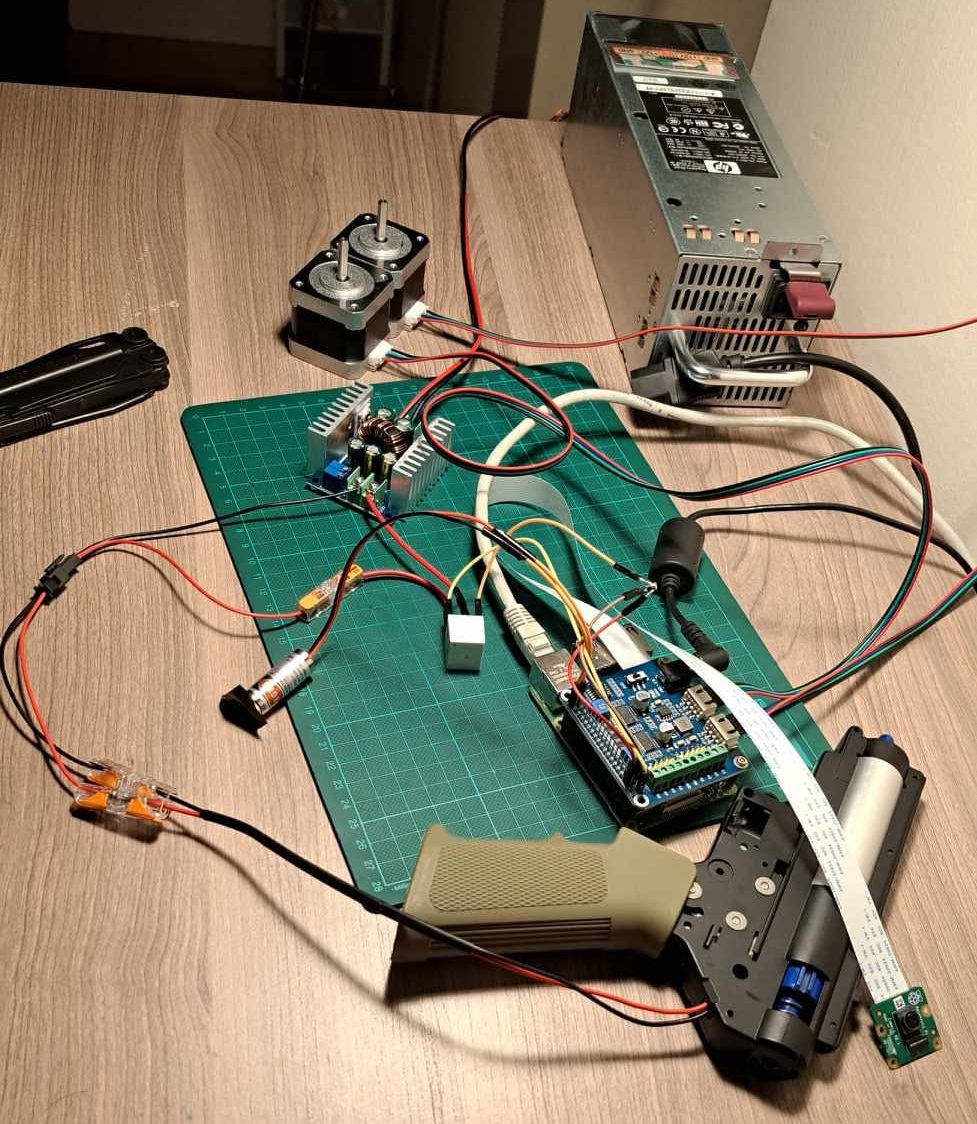
\includegraphics[width=0.6\linewidth]{teszt_1}
	\caption{Elektronikai alkatrészek teszt összeállítása}
	\label{fig:teszt_1}
\end{figure}

A teszt során azt próbáltam ki először, hogy tudom-e mozgatni a motort, működik-e a kamera, a lézer modul, tudok-e lőni a gearboxszal. Minden sikeres volt, így ezt a tesztet lezártam.

\subsection{Képfelismerő algoritmusok tesztje tesztje}
A teszt összeállítása itt is ugyanaz volt, mint az előző bekezdésben, annyi különbséggel, hogy a kamerát felerősítettem egy állványra, és egy kinyomtatott arcot mozgattam előtte. A célpont a \ref{fig:teszt_facetarget}. ábrán látható. A minta részletei nagyon kontrasztosak, elütnek egymástól, ezzel könnyítve az algoritmusok munkáját.

\begin{figure}[h!]
	\centering
	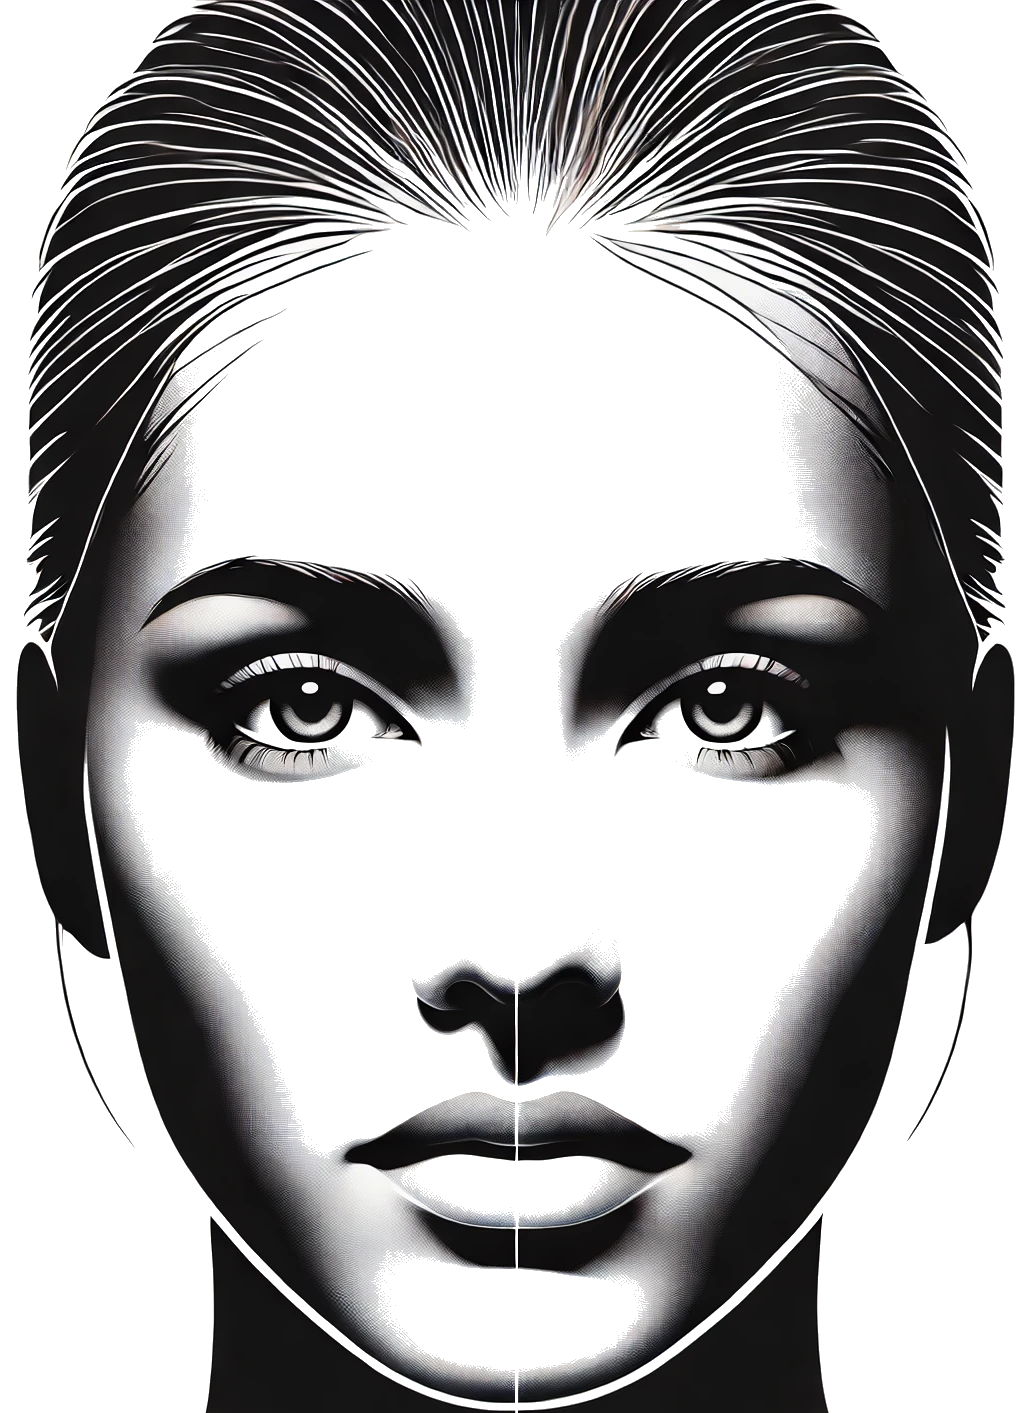
\includegraphics[width=0.6\linewidth]{facetarget1}
	\caption{Az arcfelismeréshez használt kép}
	\label{fig:teszt_facetarget}
\end{figure}

Először két olyan módszert vizsgáltam, ahol a célpont nem általános, hanem egy PNG képet vesz mintának, és ezt keresi a kamera által szolgáltatott képen.

\subsubsection*{Template Matching}
Erről a módszerről korábban a \ref{sec:soft_template}. bekezdésben írtam. A \code{cv2.matchTemplate()} függvény létrehozza megkeresi a képen sablont, a \code{cv2.minMaxLoc()} pedig visszaadja a helyzetét, valamint az eredmény pontosságát. Az eredmény pontosságának megszabtam egy alsó határt, és azt változtattam a teszt során. Azt tapasztaltam, hogy ez  a módszer nagyon érzékeny a célpont dőlésére és elfordulására, valamint a távolságára is. Semmiképpen nem optimális a feladat elvégzésére.

\subsubsection*{Feature Matching és Target Tracking}
A feature matching elviekben jól kezeli a célpont torzulását, ezért ezzel kísérleteztem a későbbiekben. 

\subsubsection*{}

\subsection{Tesztelési környezet}
A tesztet egy jól megvilágított tanteremben végeztem. Az eszköz egy stabil padon állt, a célpont pedig 5 méterrel előtte, és kb. fél méterrel fölötte. A célpont az alábbi ábrán látható:

A teszt során a manuális működési móddal kezdtem, tulajdonképpen belőttem a fegyvert. Először azt tapasztaltam, hogy a kamera képének a közepe nem ott van, ahova a fegyver csöve mutat. Ezért a célkeresztet addig kellett mozgatnom a képen, amíg oda nem mutatott, ahova a fegyver ténylegesen lőtt. Ezután azt tapasztaltam, hogy nagy pontossággal képes lőni, igen kis területen belül. A lézer irányzékot azonban nem tudtam pontosan beállítani, 5 méteren nagyjából 10-15 cm-t téved. A következő ábrákon látható a teszt eredménye. 5-ös sorozatokban tüzeltem, mindig a cél közepére irányítva a kamera célkeresztjét. \\

A következő teszt az arcfelismerés, és a követés funkció tesztje volt. A körülmények ugyanazok maradtak, és szintén 5 m-re volt a célpont. A teszt során egy kolléga tartotta a kinyomtatott arcképet, és mozgatta, változtatva a sebességet és irányt. Természetesen a gearbox nem volt áram alatt, és a kolléga is viselt védőszemüveget. Azt tapasztaltam, hogy a fegyver körülbelül a sétáló ember sebességét tudja követni 5 m távolságban, és igen pontosan be tudja célozni. A teszt az alábbi ábrán látható:
%\subsection{Teljesítménymutatók}
%a
%\subsection{Kísérleti eredmények}
%a
%\subsection{Eredmények elemzése}
%a
\section{Hibák, észrevételek}
\subsubsection{Mechanikai megvalósítás}
A
%\section{Továbbfejlesztési lehetőségek}
%a
%\section{Költségek}
%a
%\section{Konklúziók}
%a
%\section{Köszönetnyilvánítás}
%a
\pagebreak

\section*{Függelék}
\subsection*{Kódrészletek}


\pagebreak
	\begin{thebibliography}{}
	\bibitem{crows}
	Leírás a CROWS rendszerről \hfill (Hozzáférés: 2024.01.22.) \\
	{\footnotesize \url{https://www.globalsecurity.org/military/systems/ground/m101-crows.htm}},
	
	\bibitem{arbalet}
	Leírás az Arbalet-DM rendszerről \hfill (Hozzáférés: 2024.01.22.) \\
	{\footnotesize \url{http://roe.ru/eng/catalog/land-forces/RWS/arbalet-dm/}},
	
	\bibitem{defnder}
	Leírás az deFNder Medium rendszerről \hfill (Hozzáférés: 2024.01.22.) \\
	{\footnotesize \url{https://fnamerica.com/products/weapon-systems/defnder-medium/}},
	
	\bibitem{samsung}
	Leírás a Samsung SGR-A1 rendszerről \hfill (Hozzáférés: 2024.02.10.) \\
	{\footnotesize \url{https://www.globalsecurity.org/military/world/rok/sgr-a1.htm}},
	
	\bibitem{aisroftteszt}
	Teszt az airsoft gearbox áramfogyasztásáról \hfill (Hozzáférés: 2024.10.22.) \\
	{\footnotesize \url{http://www.airsoftlab.eu/docs/experiments/motor_current/}},
	
	\bibitem{nema17}
	A NEMA szabvány\hfill (Hozzáférés: 2024.10.22.) \\
	{\footnotesize \url{https://www.cncitalia.net/file/pdf/nemastandard.pdf}},
	
	\bibitem{4gbforum}
	Felhasználói diskurzus a Raspberry PI gépi látás kapacitásáról\hfill (Hozzáférés: 2024.10.22.) \\
	{\footnotesize \url{https://forums.raspberrypi.com/viewtopic.php?t=366431}},
	
	\bibitem{raspberry4}
	Raspberry 4B specifikációk\hfill (Hozzáférés: 2024.10.22.) \\
	{\footnotesize \url{https://www.raspberrypi.com/products/raspberry-pi-4-model-b/specifications/}},
	
	\bibitem{stepperhat}
	Waveshare stepper motor hat spevifikációk\hfill (Hozzáférés: 2024.10.22.) \\
	{\footnotesize \url{https://www.waveshare.com/wiki/Stepper_Motor_HAT}},

	\bibitem{raspberrycam}
	Raspberry 2 kamera specifikációk\hfill (Hozzáférés: 2024.10.22.) \\
	{\footnotesize \url{https://www.raspberrypi.com/products/camera-module-v2/}},

\end{thebibliography}


\end{document}